% =====================================================================
% main_v2.tex --- Restructured 6-section draft (skeleton)
%
%   1. Abstract + keywords
%   2. Introduction
%   3. Results              (one subsection per discovery)
%   4. Discussion
%   5. References (bibliography)
%   6. Appendix / Methods   (the "blueprint" container)
%
% Companion files:
%   - references.bib   (BibTeX, replaces the in-line thebibliography of main.tex)
%   - arxiv.sty        (unchanged, shared with main.tex)
%
% Compile sequence:
%   pdflatex main_v2.tex
%   bibtex   main_v2
%   pdflatex main_v2.tex
%   pdflatex main_v2.tex
%
% Status (2026-04-27):
%   - Abstract: drafted (v2).
%   - Introduction: PLACEHOLDER. Salvage main.tex L100-183.
%   - Results 3.1, 3.2, 3.3: drafted from main.tex with framing reset
%     (no "over-estimation", no human-LLM baseline, no causal language).
%   - Results 3.4: PLANNED (random-forest analysis pending; script
%     skeleton at src/analyze/rebuttal_rf_prediction.py).
%   - Figures 1-5: placeholder fboxes. Implementations deferred.
%   - Discussion: PLACEHOLDER.
%   - References: bibliography wired (\nocite{*} temporary).
%   - Appendix subsections: all drafted from main.tex, except
%     app:prompts (still placeholder) and app:rf-prediction (planned).
% =====================================================================

\documentclass{article}
\usepackage{pdflscape}

\usepackage{arxiv}

\usepackage[utf8]{inputenc}
\usepackage[T1]{fontenc}
\usepackage{url}
\usepackage{booktabs}
\usepackage{amsfonts}
\usepackage{nicefrac}
\usepackage{microtype}
\usepackage{multirow}
\usepackage{xcolor}
\usepackage{graphicx}
\usepackage{orcidlink}
\usepackage{array}
\newcolumntype{R}[1]{>{\raggedleft\arraybackslash}p{#1}}
\newcolumntype{L}[1]{>{\raggedright\arraybackslash}p{#1}}

\usepackage[numbers]{natbib}
\usepackage{longtable}
\usepackage{caption}
\usepackage{subcaption}
\usepackage[section]{placeins}
\usepackage{amsmath}
\usepackage{cleveref}

% ---------- Number formatting ----------
\usepackage{siunitx}
\sisetup{group-separator={,}, group-minimum-digits=4}

% ---------- Lists ----------
\usepackage{enumitem}

% ---------- Custom commands ----------
\newcommand{\code}[1]{\texttt{#1}}
\newcommand{\auc}{\text{AUC}}
\newcommand{\auprc}{\text{AUPRC}}
\usepackage{xspace}
\makeatletter
\newcommand{\ie}{i.e.\@\xspace}
\newcommand{\eg}{e.g.\@\xspace}
\makeatother

\makeatletter
\renewcommand{\footnotesize}{\@setfontsize\footnotesize{8pt}{10pt}}
\makeatother

\makeatletter
\renewcommand{\scriptsize}{\@setfontsize\scriptsize{7pt}{9pt}}
\makeatother

\definecolor{VUB_blauw}{rgb}{0.1529, 0.2667, 0.5529}
\usepackage{hyperref}
\hypersetup{
    colorlinks,%
    citecolor=VUB_blauw,%
    filecolor=VUB_blauw,%
    linkcolor=VUB_blauw,%
    urlcolor=VUB_blauw
}
\graphicspath{ {./images/}{../../data/results/figures/} }
\newcommand{\customCor}[1]{%
  
\includegraphics[height=1em]{panda2.png} #1%
}

% Lightweight keywords command (arxiv.sty does not provide one).
\providecommand{\keywords}[1]{%
  \vspace{0.5em}\noindent\textbf{Keywords:}\ #1\par\vspace{0.5em}%
}

\bibliographystyle{plainnat}

% ======================================================================
% TITLE
% ======================================================================
\title{%
  Reviewer Movability in Peer-Review Rebuttals:\\ 
  A Large-Scale Analysis of What Is Predetermined and What Author Responses Add%
}
\runningtitle{}

\author{
 Mathieu Louis\textsuperscript{1, 2, \customCor{ }} \\
    \orcidlink{0009-0003-0589-4357} \And
 Tibo Vanleke\textsuperscript{1, 2} \\
    \orcidlink{0009-0003-2200-7529} \And
    Vincent Ginis\textsuperscript{1,2,3} \\
 \orcidlink{0000-0003-0063-9608} \And
      Andres Algaba\textsuperscript{1,2} \\
 \orcidlink{0000-0002-0532-3066}\\
 \AND
  \textsuperscript{1}Data Analytics Lab, Vrije Universiteit Brussel, Pleinlaan 5, 1050 Brussel, Belgium \\
  \textsuperscript{2}imec-SMIT, Vrije Universiteit Brussel, Pleinlaan 9, 1050 Brussels, Belgium\\
  \textsuperscript{3}School of Engineering and Applied Sciences, Harvard University, Cambridge, Massachusetts 02138, USA
}

\begin{document}
\maketitle
\renewcommand{\thefootnote}{}
\footnotetext{
\includegraphics[height=1em]{panda2.png} Corresponding author: \href{mailto:mathieu.pierre.louis@vub.be}{mathieu.pierre.louis@vub.be} \\}
\renewcommand{\thefootnote}{\arabic{footnote}}
\thispagestyle{plain}

% ======================================================================
% 1. ABSTRACT + KEYWORDS
% ======================================================================
\begin{abstract}
% v2 draft (2026-04-27). ~240 words. Structure: setup, instrument,
% three findings in Results-section order, synthesis. Constraints:
% no em dashes, no semicolons, no causal language, no banned hedges,
% "LLM-detected text-vs-score gap" framing not "over-estimation".
% v2 change: removed the human inter-reviewer comparison (32.7/77.3)
% --- different task (independent scoring vs. text decoding), not
% a valid baseline for Gemini. See feedback memory
% `feedback_no_human_llm_baseline_compare.md`.

Peer review gates which scientific work gets published, and the rebuttal is the one window in which authors can respond to reviewer concerns and reviewers can revise their scores before a final decision. Whether and how rebuttals actually shift scores has been hard to study at scale, since the substantive content of reviewer-author exchanges is rarely measured directly. We analyze \num{73000} ICLR 2024--2025 reviews linked to external pre- and post-rebuttal scores, asking how much score movement is already predictable before rebuttal and how much is added by the author response. A Gemini Flash 3 score decoder applied to score-stripped review text yields a text-score residual that predicts later movement: score-increase rates rise from 8\% when the model reads the text below the assigned score, to 19\% when they match, to 32\% when the text reads above the score. We then induce a 44-factor rebuttal taxonomy with Claude and classify rebuttal threads with Gemini. In temporal validation, pre-rebuttal features alone reach AUC $0.744$, dominated by the focal reviewer's initial score, the paper-level initial mean, and the contribution sub-score. Adding rebuttal-content features raises AUC to $0.801$, while post-discussion co-reviewer movement adds only $0.005$. The content gain is largest for near-consensus reviewers ($+0.090$ AUC), smaller for below-mean reviewers ($+0.069$), and smallest for above-mean reviewers ($+0.046$). The strongest content signals are unresolved concerns: persistent clarity problems, methodological weaknesses, weak novelty justification, insufficient evidence, and defensive tone. Rebuttal success is therefore neither simple persuasion nor predetermined outcome: initial reviewer-paper structure creates a movability envelope, and rebuttal content adds bounded but real signal inside it.

\end{abstract}

\keywords{peer review, large language models, rebuttal dynamics, score prediction, reviewer behaviour}

% ======================================================================
% 2. INTRODUCTION
% ======================================================================
\section{Introduction}\label{sec:intro}

Peer review at large machine-learning conferences is the principal quality-control mechanism for the field, and it is showing signs of strain. ICLR submissions grew from \num{4955} in 2023 to \num{19814} in 2026, a roughly four-fold increase in four years~\cite{papercopilot}. The 2014 NeurIPS experiment, which assigned the same papers to two independent program committees, found that about 25 percent of accept/reject decisions were inconsistent across committees~\cite{cortes}. Surveys of biomedical reviewers report that a small share of the community absorbs the bulk of the load~\cite{kovanis,adam}. These are different facets of the same operational problem: submission volume has outpaced reviewer supply, leaving accept/reject decisions visibly noisy and reviewing effort unevenly distributed.

This paper takes on the question of what governs whether reviewers revise their scores during the rebuttal phase. We decompose post-rebuttal score change into pre-rebuttal predictability and rebuttal-content lift on \num{73000} ICLR 2024--2025 reviews, building two measurement instruments along the way: an LLM-derived text-vs-score offset that exposes within-review variability invisible to the numeric rating alone, and a 44-factor rebuttal-content codebook with declared polarity, validated cross-model and cross-year. Pre-rebuttal features alone reach $\auc = 0.744$ on a temporal split, and adding rebuttal-content features lifts $\auc$ to $0.801$, with the content gain concentrated among reviewers near the paper-level initial mean. Concurrent work by Kargaran et al.~\cite{kargaran} reports related structural correlates on overlapping data. Our distinct contributions are the controlled decomposition into pre-rebuttal envelope and content lift, the asymmetric positive-vs-negative polarity screen the codebook enables, and the within-review text-vs-score residual as a per-reviewer signal.

Within this process, the rebuttal and discussion phase on OpenReview is the only window in which authors can respond to concerns and reviewers can update their numeric scores before the final decision. The phase is consequential. Across ICLR 2024 and 2025, $21\%$ of reviewers raised their score after rebuttal and $1.4\%$ lowered it ($n = \num{73000}$). Yet what governs whether a reviewer revises a score during this window has been hard to study at scale. Prior work has identified structural correlates of review and rebuttal outcomes, including thread length and depth, response latency, review submission timing, and signed-network co-reviewer effects~\cite{huang,jung,kargaran}. Earlier NLP corpora have built foundational annotations of peer-review discourse (PeerRead~\cite{kang}, AMPERE~\cite{hua}, DISAPERE~\cite{kennard}), with Kuznetsov et al.~\cite{kuznetsov} providing a recent survey. Methodology for testing reviewer-side biases has been developed via randomised paper-assignment designs~\cite{stelmakh}. The substantive content of reviewer-author exchanges has not been measured systematically at this scale, however, particularly with a declared-polarity factor codebook operationalisable by an independent LLM. Our analysis controls for thread length (rebuttal length and number of author replies, plus the full thread-message count at the post-discussion horizon), thread-structure and timing features following Jung et al.~\cite{jung} (maximum dialogue-tree depth, the days from review submission to the first author reply, and the days from review submission to the official ICLR review-submission deadline), alongside the initial-review structural fields the OpenReview dataset exposes. We do not isolate reviewer workload because reviewer identifiers on OpenReview are anonymised at the paper level and cannot be linked across papers, a limitation the cited prior work shares.

Recent work has begun using large language models inside peer review. Liang et al.~\cite{liang} showed that LLMs can produce useful feedback on research papers, and Thakkar et al.~\cite{thakkar} reported a randomised intervention in which LLM feedback improved human-written reviews on more than 20{,}000 ICLR 2025 reviews. This intervention overlaps with the ICLR 2025 portion of our corpus, a contamination we acknowledge and discuss in \Cref{sec:discussion}. The broader LLM-as-judge literature also documents position, verbosity, and self-enhancement biases that complicate the use of LLMs as evaluation oracles~\cite{zheng}. These deployments treat the LLM as a writing tool or judge. We instead use LLMs as measurement instruments on existing review text: one model decodes a numeric score from score-stripped review wording, and we use the residual between that decoded score and the reviewer's assigned score as a within-review signal. A second, independent model classifies rebuttal threads against a fixed 44-factor taxonomy that we first induce from a separate sample. In both cases the output is a measurement of what reviewers and authors wrote, not text generated for them. Together, these measurements let us ask how much score movement is already predictable before rebuttal, and how much additional signal appears once the rebuttal exchange is observed.

Our main finding is simple: a rebuttal is neither pure persuasion nor a foregone conclusion. Reviewers arrive at the rebuttal phase with different amounts of room to move. That room depends on the score they gave, how it compares to their co-reviewers, and how the paper looks overall at that point. What the rebuttal actually says still matters on top of these starting conditions. The effect is largest for reviewers near the middle of the pack. These are the cases where the outcome is least clear at the start.

We analyze \num{73000} reviews from \num{18400} ICLR 2024 and 2025 papers paired with externally archived pre- and post-rebuttal scores from~\cite{kargaran}. The rebuttal-content analysis uses a \num{6705}-rebuttal cohort with both Gemini Flash 3 score predictions and parsed factor labels. The analyses supporting the movability-envelope claim proceed in four steps.

\textbf{\Cref{res:instrument}} validates Gemini Flash 3 as a measurement instrument. Its score predictions span the ICLR scale, and the LLM-derived text-score residual predicts later score movement: post-rebuttal increase rates rise from $8\%$ when the model reads the text below the assigned score, to $19\%$ when they match, to $32\%$ when the text reads above the score.

\textbf{\Cref{res:rebuttal-categories}} induces a 44-factor rebuttal taxonomy with Claude on a stratified \num{1000}-interaction ICLR 2025 sample, then validates the fixed codebook with a separate outcome-blinded Gemini Flash 3 classification run on both the induction sample and a held-out \num{5730}-interaction ICLR 2024 cohort. Twenty-three factors cross the family-wise-error Bonferroni-corrected threshold ($\alpha = 0.05/44$) in both tests and form the conservative core of the taxonomy. Under the less conservative Benjamini-Hochberg false-discovery-rate threshold ($q = 0.05$), 31 of 44 are significant in both tests (\Cref{app:horizons}).

\textbf{\Cref{sec:horizons}} asks which rebuttal behaviours remain associated with score increase after controlling for reviewer-paper structure. A paper-clustered logistic model identifies five positive and ten negative factors that meet a robust association screen. The dominant signal, however, is structural rather than rhetorical: reviewers below the paper-level initial mean are far more likely to increase than reviewers already above it. Rebuttal-content factors retain their direction within movability strata, but their interpretation is conditional on this baseline structure.

\textbf{\Cref{sec:rebuttal-impact}} quantifies the predictive contribution of rebuttal content across authoring horizons. Pre-rebuttal features alone reach $\auc = 0.744$ on a temporal split (train ICLR 2024, test ICLR 2025). Adding rebuttal-content features lifts $\auc$ to $0.801$, while post-discussion co-reviewer movement adds only $+0.005$ on top. The content gain is heterogeneous: it is largest for near-consensus reviewers, smaller for below-mean reviewers, and smallest for above-mean reviewers. The strongest content signals are negative: persistent clarity problems, unresolved methodological concerns, weak novelty justification, insufficient evidence, and defensive tone.

The remainder of the paper develops these analyses in order. \Cref{sec:results} presents the measurement instruments, rebuttal taxonomy, controlled associations, and horizon models. \Cref{sec:discussion} discusses what the results imply for venues, reviewers, and authors, and what they do not warrant.


% ======================================================================
% 3. RESULTS
% ======================================================================
\section{Results}\label{sec:results}

% ----------------------------------------------------------------------
% Figure 1 --- methodology + key discoveries (overview)
% ----------------------------------------------------------------------
%
% SPECIFICATION (implementation deferred):
%
%   Layout (landscape, ~2:1 aspect ratio):
%
%     ROW A --- PIPELINE (full width, ~40% height)
%       [ICLR 2024+2025 (~73K reviews + external GT)]
%         -> [Gemini Flash 3: initial-score prediction + content coding]
%         -> [Score-change verdicts (Gemini 89.6% vs. regex 73.1%)]
%         -> [Trigger / mediation analyses]
%
%     ROW B --- KEY DISCOVERIES (4 mini-panels, ~60% height)
%     Aligned with the four Results subsections (3.1--3.4):
%       D1. LLM as instrument:   40.7% exact / 87.6% within 1 step,
%                                + text-vs-score gap funnel
%                                (8% under, 19% matched, 32% over)
%       D2. Rebuttal categories: heatmap of category x tier ORs;
%                                "new experiments" strongest
%       D3. Inference (M1-M8 +   M4=0.785 -> M8=0.791;
%           triggers):           rebuttal effort, peer movement,
%                                outlier x confidence as headlines
%       D4. Prediction ceiling:  RF vs logistic (PLANNED)
%
%   Build with src/core/plot_theme.py (setup_publication_theme,
%   Okabe-Ito palette). Source numbers all already exist under
%   data/results/{gemini_prediction,overestimation_analysis,
%   prediction_comparison,confidence_triggers}/.
%   Save target: data/results/figures/figure1_overview.{png,pdf}.
%   Implementation reference: notebooks/hero_figure.py.
%
% ----------------------------------------------------------------------
\begin{figure}[t]
  \centering
  % \includegraphics[width=\linewidth]{figure1_overview.pdf}
  \fbox{\parbox[c][6cm][c]{0.95\linewidth}{\centering \textit{Figure 1 placeholder ---
    methodology pipeline (top) and four key discoveries (bottom).
    See specification in source comments above; implementation deferred.}}}
  \caption{\textbf{Overview of the study.} (Top) Analysis pipeline:
    raw OpenReview submissions are normalised, scored by Gemini Flash 3,
    cross-checked against an external pre/post-rebuttal ground truth, and
    fed into trigger and mediation analyses. (Bottom) Headline results
    for the four discoveries reported in this paper.}
  \label{fig:f1-overview}
\end{figure}

% ======================================================================
% NEW Results structure (locked 2026-04-27 with user):
%
%   3.1 LLM as instrument: Gemini decodes initial reviewer scores from
%       review text (40.7 / 87.6) and reveals a within-review text-vs-
%       score gap that itself predicts post-rebuttal increases.
%   3.2 LLM-derived categories of successful and unsuccessful rebuttals.
%   3.3 Inference: an 8-model paper-clustered logistic ladder identifies
%       which factors are associated with score increase, controlling
%       for confounders (rebuttal effort, peer movement, outlier x
%       confidence as the headline associations).
%   3.4 Prediction: random-forest predictive ceiling, comparing against
%       the linear inference model. (PLANNED ANALYSIS.)
%
%   Operational definition of "successful rebuttal" (locked 2026-04-27):
%   binary outcome = ext_direction == "increase" (post-rebuttal score
%   strictly higher than ext_rating_before). Used consistently in
%   3.2, 3.3, 3.4. Alternative outcomes (paper accepted, magnitude of
%   increase, reviewer engagement uptick) deferred to future work.
% ======================================================================

% ----------------------------------------------------------------------
% 3.1 LLM as instrument: score decoding + text-vs-score gap.
% Combines old res:prediction (instrument validation) with old
% res:text-score-gap (the calibration signal the instrument exposes).
% ----------------------------------------------------------------------
\subsection{Gemini Flash 3 decodes reviewer scores from text, and the residual gap to the assigned score predicts post-rebuttal increases}\label{res:instrument}
% PLACEHOLDER --- one paragraph in a later session.
%
% IMPORTANT framing note (do NOT regress on this):
%   This subsection is INSTRUMENT VALIDATION, not a comparison against human reviewers. Gemini reads the review text (which already contains the rationale, sub-scores, weaknesses, and questions the reviewer
%   wrote alongside the score), so its task is decoding text -> score.
%   Human inter-reviewer agreement (32.7 / 77.3) measures a DIFFERENT
%   task: two reviewers independently scoring the same paper with no
%   shared text. The two numbers are not comparable as baseline-vs-system
%   and we do NOT claim Gemini "exceeds" the human baseline.
%   The human-human number is reported separately in
%   Appendix \ref{app:reviewer-agree} as evidence that review scoring is
%   itself noisy, not as a Gemini baseline.
%
% (a) Score-decoding accuracy (instrument validation).
%   What we did: predicted the initial pre-rebuttal score from review
%     text alone on n=\num{73000} reviews (ICLR 2024+2025) with Gemini
%     Flash 3, validated against ext_rating_before (PaperCopilot /
%     Kargaran et al.).
%   What we found: 40.7\% exact match, 87.6\% within 1 step (combined),
%     sufficient to use Gemini as a measurement instrument for the
%     analyses in 3.2--3.4.
%
% (b) Text-vs-score gap (a calibration signal the instrument exposes).
%   What we did: defined offset = (Gemini-predicted score from text)
%     minus (actual assigned initial score). Measured post-rebuttal
%     score-increase rate as a function of offset.
%   What we found: monotonic gradient. Combined under 8.3\% increase,
%     matched 19.2\%, over 31.9\% (n=73,000). Direction replicates in
%     2024 and 2025; magnitude is larger in 2025 (8.5 -> 35.8) than in
%     2024 (7.9 -> 26.1) (funnel\_stats.csv). Mediation through
%     engagement quality only 5.2\%
%     (combined\_20242025\_mediation.csv), so the signal is largely
%     independent of stance and engagement.
%   Caveats: "LLM-detected" is doing real work --- no non-LLM gold
%     standard for what review text should imply. Predictive, not
%     causal. Multivariate marginal contribution is small once paper-
%     mean position is controlled (see \Cref{sec:horizons}).
%
% Reference: \Cref{fig:f2-instrument}; details in
%   \Cref{app:gemini-pred,app:ext-gt,app:text-score-gap}.
%   (Inter-reviewer agreement reported separately in
%   \Cref{app:reviewer-agree}, NOT as a Gemini baseline.)

We evaluate Gemini Flash 3 as a measurement instrument on two tasks: decoding initial reviewer scores from review text alone, and using the gap between this LLM-decoded score and the score the reviewer actually assigned (the \emph{text-vs-score gap}) as a within-review signal that itself predicts post-rebuttal increases. We submitted all ICLR 2024 and 2025 reviews to the Gemini Batch API after stripping every numeric scoring field that the reviewer fills in (\code{soundness}, \code{presentation}, \code{contribution}, \code{rating}, \code{recommendation}, and the reviewer's self-reported \code{confidence} on the 1--5 scale to prevent leakage of the answer into the input (\Cref{app:gemini-pred}). The model was asked for an inferred score on the six-point ICLR scale, together with an inferred reviewer confidence, sentiment, and engagement-quality ratings. Across \num{73000} reviews, Gemini's predictions span the full ICLR scale --- 19\% of predictions at score 3, 46\% at 5, 27\% at 6, 7\% at 8 --- and roughly mirror the assigned-score distribution (30\% / 35\% / 24\% / 9\% respectively), so the model is not collapsed onto a single value. Gemini's decoded score matches the reviewer's assigned score in 40.7\% of reviews. In the remaining 59.3\% the LLM reads the text as below the assigned score (24.3\%) or above it (35.0\%), with mean offset $+0.14$ steps and SD $1.02$. There is therefore per-review variability for downstream analyses to use. Rank-order correlation provides a sanity check that this offset has interpretable directionality rather than being random noise: predictions and assigned scores are monotonically associated (combined Spearman $\rho = 0.40$, \Cref{app:gemini-pred}). The instrument is best characterised as moderate at agreeing with the reviewer ($\rho = 0.40$, exact-match $40.7\%$) but informative at extracting per-review residual. The downstream analyses do not require Gemini to agree with the reviewer. They require the disagreement to carry information, which a constant-mode predictor of the score is structurally incapable of producing. The score-adjustment validation confirms the model is decoding the \emph{initial} score, not the final one: adjusting predictions by the detected change direction improves accuracy. This is expected, since the model reads review text written before any rebuttal. The decisive instrument-validation evidence is in the next paragraph: the per-review offset predicts post-rebuttal increase rates of 8\% / 19\% / 32\% across the offset gradient, a within-review signal a constant predictor of the score is structurally incapable of producing.

The same prompt also requested an inferred reviewer confidence on the 1--5 scale, but unlike the score, that secondary output \emph{is} essentially collapsed onto a single value. Gemini predicts confidence 4 in 80\% of cases against a true rate of 47\%, and its prediction distribution barely tracks the underlying spread (1.7\% / 7.6\% on confidences 1--2 in the input vs.\ 2.6\% in predictions, and 13\% on confidence 5 in the input vs.\ 7\% in predictions). Rank-order association with the held-out self-reported confidence is correspondingly weak (combined Spearman $\rho = 0.18$, mostly carried by ICLR 2024 at $\rho = 0.29$, with ICLR 2025 alone at $\rho = 0.06$). The contrast with the score result is the right comparison: per-review information is what we extract from the score channel and what we cannot extract from the confidence channel, so no analog to the offset funnel exists for confidence. We therefore use only the inferred score in the analyses that follow (\Cref{app:gemini-pred}).

The same instrument exposes a within-review text-vs-score gap. We define the \emph{offset} as the Gemini-decoded score minus the actually assigned initial score, measured in \emph{step positions} on the six-point ICLR ladder $\{1, 3, 5, 6, 8, 10\}$ rather than in raw points, since the ladder has uneven gaps (\Cref{app:gemini-pred}). A reviewer who scored a paper $5$ while Gemini decoded the text as a $6$ thus has offset $+1$ step, identical to a reviewer who scored $3$ while Gemini decoded a $5$. Across \num{73000} reviews with both Gemini predictions and external ground truth, post-rebuttal score-increase rate rises monotonically with offset: 8.3\% for reviews where the LLM read the text as below the assigned score, 19.2\% for reviews where the two agreed, and 31.9\% for reviews where the LLM read the text as above the assigned score. The direction of this gradient replicates in both years. The magnitude is larger in 2025 (8.5\% to 35.8\%) than in 2024 (7.9\% to 26.1\%) (\code{funnel\_stats.csv}). The mirror gradient runs for the (much rarer) post-rebuttal decreases: 3.3\% in the under-offset bin, 1.0\% at zero offset, and 0.4\% in the over-offset bin, against a 1.4\% baseline overall. The offset therefore captures bidirectional score volatility, with under-offset reviewers about eight times more likely to revise down than over-offset reviewers, and over-offset reviewers about four times more likely to revise up than under-offset reviewers. Both directions are consistent with a reading where the offset measures tension between the substantive critique and the numeric verdict, and the rebuttal is the moment that tension gets resolved. We checked whether the offset's predictive value runs through any of the auxiliary per-review ratings Gemini also produced (engagement-quality, sentiment, tone) rather than reflecting something specific to the text-vs-score gap itself. Adding all three jointly as covariates in a logistic increase model shrinks the offset coefficient from $0.643$ to $0.492$, a 23.6\% reduction (\Cref{app:text-score-gap} for per-mediator decompositions and methodology). About three-quarters of the offset's predictive effect on post-rebuttal increase is therefore unaccounted for by any of these alternative text-derived ratings. Three caveats apply throughout. First, ``LLM-detected'' is doing real work: we have no non-LLM gold standard for what review text should imply, so the offset is a property of the LLM's decoding rather than an objective measure of textual positivity. Second, the relationship is predictive, not causal. Third, the multivariate marginal contribution of the offset is small once paper-mean position is controlled (\Cref{sec:horizons}).


\begin{figure}[!htb]
  \centering
  \begin{subfigure}[b]{0.49\linewidth}
    \centering
    \includegraphics[width=\linewidth]{../../data/results/gemini_prediction/figures/gemini_pred_combined_confusion_initial.pdf}
    \caption{Score-decoding accuracy}
    \label{fig:f2-confusion}
  \end{subfigure}\hfill
  \begin{subfigure}[b]{0.49\linewidth}
    \centering
    \includegraphics[width=\linewidth]{../../data/results/gemini_prediction/figures/funnel_increase_rate.pdf}
    \caption{Text-vs-score-gap funnel}
    \label{fig:f2-funnel}
  \end{subfigure}
  \caption{\textbf{Gemini Flash 3 as instrument: score decoding and the within-review calibration signal.} (\subref{fig:f2-confusion}) Row-normalised confusion matrix of Gemini-decoded initial reviewer scores against the external pre-rebuttal ground truth on the combined ICLR 2024+2025 cohort ($n = \num{73000}$): exact-match $40.7\%$, within-1 $87.6\%$, Spearman $\rho = 0.40$, mean bias $+0.14$ steps. (\subref{fig:f2-funnel}) Post-rebuttal score-increase rate as a function of the Gemini text-vs-score offset bucket. Combined bars rise monotonically ($8.3\% \to 19.2\% \to 31.9\%$) and the gradient replicates in both years (markers); the 2025 magnitude is larger ($8.5\% \to 35.8\%$) than the 2024 magnitude ($7.9\% \to 26.1\%$).}
  \label{fig:f2-instrument}
\end{figure}

% ----------------------------------------------------------------------
% 3.2 LLM-derived categories of successful and unsuccessful rebuttals.
% (PROMOTED from appendix --- previously only in app:rebuttal-coding.)
% ----------------------------------------------------------------------
\subsection{LLM-derived content categories distinguish successful from unsuccessful rebuttals across initial-score tiers}\label{res:rebuttal-categories}
% PLACEHOLDER --- one paragraph in a later session.
% Outcome: post-rebuttal score increase (ext_direction == "increase"), binary.
% What we did: used Gemini and Claude (categorization\_prompt.py) to tag
%   rebuttal interactions across 8 content categories (new experiments /
%   baselines, clarification / misunderstanding, novelty reframing,
%   writing / presentation fixes, theoretical additions, evaluation
%   improvements, reproducibility artifacts, scope narrowing). Computed
%   odds ratios for each category x initial-score tier (low 1-3,
%   mid 5-6, high 8-10) against the score-increase outcome. N=\num{20288}
%   interactions, ICLR 2024+2025 combined.
% What we found (category_associations_combined.csv):
%   - "New experiments / baselines" is the strongest associated category
%     at low and mid tiers (OR=1.73 low, 1.48 mid, 2.04 high; Bonferroni-
%     significant at low and mid).
%   - "Writing / presentation fixes" and "theoretical additions" also
%     have OR>1 at low and mid tiers (Bonferroni-significant in mid).
%   - The high tier has the smallest n and the noisiest ORs. Few
%     associations are Bonferroni-significant there.
% Cross-year replication (definition: same direction of OR in 2024 and
%   2025, computed from category_associations_{2024,2025}.csv):
%   - 8 categories x 3 tiers = 24 cells full grid.
%   - 23 cells present in both year files (high x scope_narrowing has
%     too few high-tier interactions to compute).
%   - 21 cells with a computable OR in both years (high x
%     {evaluation_improvements, novelty_reframing} have OR=NaN in 2024
%     due to small high-tier counts).
%   - 18 of 21 (86\%) show same-direction OR across 2024 and 2025.
%   - 3 of 23 are Bonferroni-significant in BOTH years (much stricter).
% Reference: \Cref{fig:f3-categories}; details in
%   \Cref{app:rebuttal-coding,app:prompts}.

We induced a taxonomy of rebuttal moves directly from the data using two large language models in distinct roles. Both models worked from raw thread text rather than from any structured extraction: each \emph{interaction} concatenates the full original review (summary, strengths, weaknesses, questions), the full author rebuttal, and any reviewer follow-up comments, in chronological order. A first model (Claude, hereafter LLM-A) was given a stratified sample of \num{1000} ICLR 2025 reviewer-author interactions in this raw form, arranged into six cells (initial-score tier $\times$ rebuttal outcome, where outcome is binary: \emph{increase} versus \emph{same\_decrease}), and asked to perform a within-tier contrastive analysis. The procedure was repeated five times to attenuate run-to-run variability, and the extracted categories were aggregated across runs and tiers, yielding 44 factors with a declared polarity (positive or negative). To rule out the hypothesis that LLM-A was retrieving canonical ``good rebuttal'' patterns from its prior, we re-ran the induction under two memory-control manipulations: a tier swap and a silent outcome-label swap on the same \num{1000} interactions. In both swaps the resulting factor content tracked the input data rather than the presented labels, consistent with extraction from the interaction text rather than retrieval (\Cref{app:rebuttal-coding}).

A second, independent model (Gemini Flash 3, LLM-B) then classified each interaction against the fixed 44-factor list under an outcome-blinded protocol with shuffled factor identifiers, blocking both label leakage and ordering cues. For every factor we computed an odds ratio comparing the \emph{increase} and \emph{same\_decrease} outcome groups, with a 95\% confidence interval, plus a two-sided permutation test with 2000 permutations. Significance is reported at the Bonferroni-corrected threshold $\alpha = 0.05/44 = 0.0011$, alongside the less conservative Benjamini-Hochberg false-discovery-rate threshold $q = 0.05$. The Bonferroni rule controls the family-wise error rate and is the appropriate gate for the recommendation list, where false positives lead authors to bake spurious factors into their drafts. The BH rule is reported as a sensitivity for the broader taxonomy. We ran two tests: Test 1 applied LLM-B to the same \num{1000} ICLR 2025 interactions used for induction (operationalisability by an independent model), and Test 2 applied the same protocol to the full classified ICLR 2024 cohort of \num{5730} interactions disjoint from the induction corpus (discriminative validity on fresh data). Test 1 preserves 43 of 44 codebook polarities (22 of 23 positive and 21 of 21 negative) and Test 2 preserves all 44 (23 of 23 positive and 21 of 21 negative). Twenty-three factors (9 positive, 14 negative) cross the Bonferroni threshold in \emph{both} tests and form the conservative core of the taxonomy. Switching to BH q = 0.05 in both tests adds 8 further factors and brings the doubly-significant set to 31 of 44. The 4 additional positives are $F_{08}$ acknowledging valid points, $F_{09}$ comprehensive coverage, $F_{16}$ conceptual explanations alongside empirical results, and $F_{19}$ writing fixes. The 4 additional negatives are $F_{26}$ missing reproducibility details, $F_{34}$ silent acceptance of limitations, $F_{37}$ brevity or low-effort rebuttal, and $F_{44}$ surfacing problems without proactive framing. The doubly-significant positive factors include sincere engagement (length, detail, supplementary content), concrete empirical evidence tied to reviewer concerns, baseline completion, methodological detail, explicit revision commitments, and active dialogue. The doubly-significant negative factors include defensive or evasive responses, superficial concern addressal, lack of empirical evidence, weak novelty justification, missing baseline comparisons, vague future-oriented promises, and section-referencing instead of real clarification.

\begin{figure}[!htb]
  \centering
  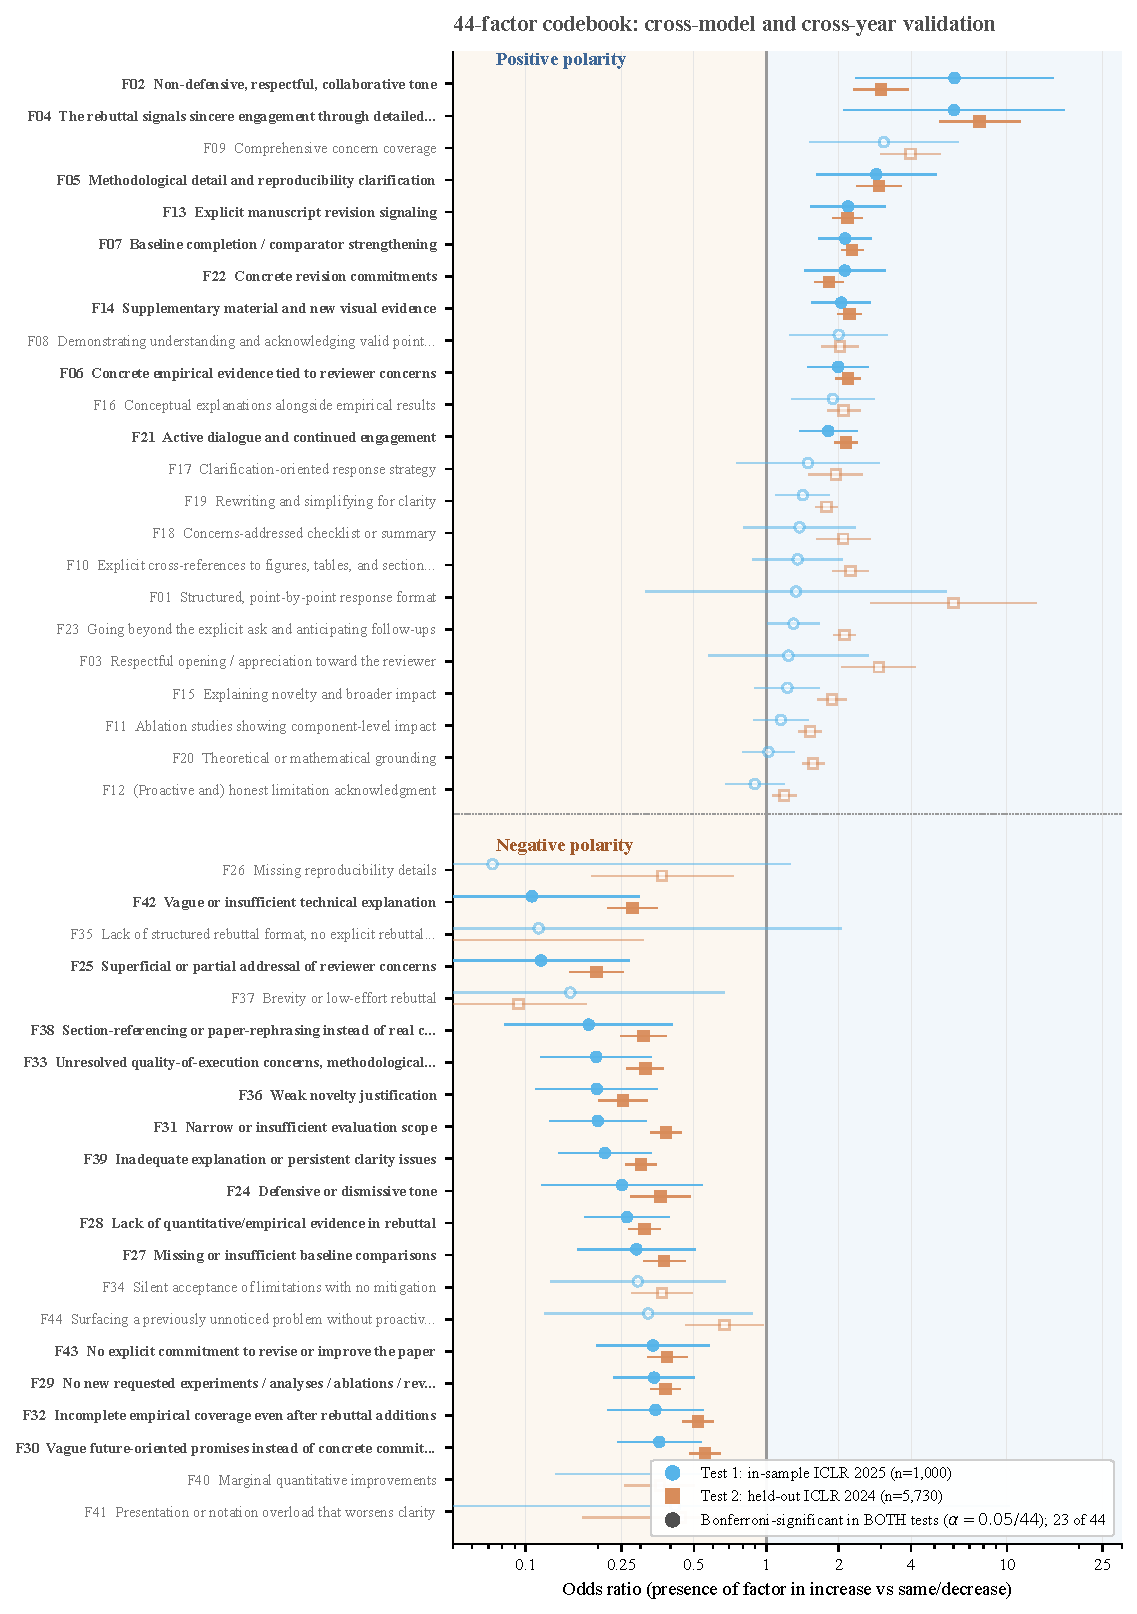
\includegraphics[width=0.78\linewidth]{../../data/results/factor_validation/figures/factor_validation_forest.pdf}
  \caption{\textbf{Claude-induced 44-factor taxonomy validated by independent
    Gemini classification.} Forest plot of all 44 codebook factors with
    odds ratios and 95\% CIs from Test 1 (in-sample, $n = \num{1000}$
    ICLR 2025, blue circles) and Test 2 (held-out full classified ICLR 2024 cohort,
    $n = \num{5730}$, orange squares). The 23 factors that cross the
    Bonferroni-corrected threshold ($\alpha = 0.05/44 = 0.0011$) in both
    tests are highlighted in bold with filled markers as the conservative
    core; the remaining factors are shown in lighter shade so the reader
    sees the continuous effect-size evidence without a dichotomised
    in/out view. Vertical line at OR = 1 marks the null. Positives
    appear in the upper block, negatives in the lower block. Memory-control
    analyses on the induction sample (\Cref{app:rebuttal-coding}) confirm
    that factor content tracks the underlying data rather than the
    presented outcome labels, consistent with extraction from the
    interaction text rather than retrieval from the model's prior.}
  \label{fig:f3-categories}
\end{figure}



% ----------------------------------------------------------------------
% 3.3 Inferential analysis. Asks: controlling for who the reviewer is
% and what the paper looks like at the time of the initial review,
% which rebuttal-content behaviors remain independently associated
% with a post-rebuttal score increase? Recommendation list as
% deliverable.
% ----------------------------------------------------------------------
\subsection{Which rebuttal behaviors are independently associated with score increase}\label{sec:horizons}

\Cref{res:instrument} established that the LLM-decoded text-vs-score offset carries within-review signal humans do not telegraph in their numeric rating. \Cref{res:rebuttal-categories} extracted that signal as a 44-factor codebook with declared polarity, validated cross-model and cross-year. We now ask the conditional question that bears on rebuttal authoring: \emph{controlling for who the reviewer is and what the paper looks like at the time of the initial review, which rebuttal-content behaviors remain independently associated with a post-rebuttal score increase?} We fit a paper-clustered logistic regression on the combined 2024+2025 rebuttal cohort ($n = 6{,}705$, base rate $45.6\%$) that regresses score-increase on the 44 factor indicators alongside ten structural confounders visible at initial-review time and four rebuttal-side aggregates whose construction tracks prior structural-correlate analyses~\cite{huang,jung,kargaran}. \Cref{app:horizons} carries the full feature catalogue, the leakage audit, and the asymmetric screen rules used to gate the recommendation list. The 44-factor family is corrected at the Bonferroni threshold $\alpha = 0.05/44 = 0.0011$.

Positive and negative factors anti-correlate within rebuttals. A draft that does $F_{07}$ baseline completion rarely also does $F_{33}$ superficial concern addressal, so the two polarity blocks compete for variance in a single joint fit and the positive-side coefficients are crowded toward zero. We therefore screen positives and negatives separately (\Cref{app:horizons}) and accept a factor as robustly associated with score increase if it meets both a univariate marginal screen and a polarity-isolated joint screen, with both 95\% CIs excluding $1$. Four of 23 codebook positives and ten of 21 codebook negatives qualify (\Cref{fig:recforest}). On the positive side the strongest individual association is $F_{07}$ baseline completion (OR $= 1.64$ [$1.42$, $1.89$], the only positive that crosses Bonferroni in the headline joint), followed by $F_{02}$ ($1.51$), $F_{19}$ writing fixes ($1.27$), and $F_{20}$ theoretical additions ($1.18$). On the negative side $F_{39}$ defensive or evasive responses (OR $= 0.31$ [$0.25$, $0.39$]) and $F_{37}$ unsatisfactory revision evidence ($0.38$) lead, followed by $F_{24}$, $F_{36}$ section-referencing instead of clarifying, $F_{33}$ superficial concern addressal, $F_{40}$, $F_{28}$, $F_{43}$, $F_{32}$, and $F_{25}$. Seven of these ten clear Bonferroni in the headline joint as well. The codebook polarity is preserved overall: a binomial sign test rejects chance at $p = 0.026$ on the positive side and $p = 0.0038$ on the negative side, with both polarity-isolated refits described in \Cref{app:horizons} reaching $p < 10^{-6}$.

The structural confounders carry effect sizes that dwarf the per-factor associations, as expected. Initial-score position is the largest single contributor (per 1 SD, OR $= 0.143$ [$0.123$, $0.165$]: high initial scores cannot rise), followed by paper-level initial mean (OR $= 1.87$ [$1.71$, $2.05$]) and the substantive sub-score \code{contribution} (OR $= 1.70$). The Gemini text-vs-score offset of \Cref{res:instrument} survives as an independent conditional contributor (OR $= 1.16$ [$1.06$, $1.26$]) even after the 44 factors are controlled. Among the prior-work structural correlates~\cite{huang,jung,kargaran}, two carry independently significant associations in the joint. \emph{Max thread depth} dominates (OR $= 1.24$ [$1.16$, $1.34$], Bonferroni-significant), consistent with deeper back-and-forth dialogue tracking richer engagement. \emph{Days remaining until the deadline} when the review was submitted is also significant (per 1 SD $\approx 4.7$ days, OR $= 1.19$ [$1.04$, $1.36$], $p = 0.011$), consistent with earlier-submitted reviews coming from more engaged reviewers who are then more open to updating after rebuttal. Rebuttal length and the number of author replies are flatly indistinguishable from $1$ in the joint specification (per 1 SD ORs of $1.02$ and $0.95$, both $p > 0.4$). First-reply latency trends toward a small negative association (per 1 SD OR $= 0.90$, $p = 0.12$) without clearing conventional significance. We have $80\%$ power against per-SD ORs $\geq 1.20$ in this design under cluster-robust SEs at $n = 6{,}705$ (\Cref{app:horizons}, \code{null\_triplet\_mde.csv}), so the nulls rule out moderate effects but not small ones. Their marginal effects in earlier work are absorbed by the rebuttal-content block in our joint specification. The same is true of the Gemini engagement rating: on its own it predicts post-rebuttal increase well (OR per SD $= 1.30$, $p < 10^{-4}$), but it loses that effect once the 44 rebuttal factors are in the model (OR $= 1.04$, $p = 0.44$). The factors capture the same signal in finer detail. Two ablations reported in \Cref{app:horizons} confirm the screen is not artefactual. Dropping all structural confounders shifts factor ORs by a median $5.4\%$ with polarity preserved, and stratum fixed effects on $46$ (deviation $\times$ initial-score $\times$ confidence) cells preserve magnitudes within $2.8\%$.

The single largest predictor of post-rebuttal increase is structural rather than rhetorical: a reviewer who scored a paper below its initial co-reviewer mean has more headroom and more social-inferential pressure to revise upward than one who already scored at or above the mean. Pre-rebuttal predictability is not, however, mechanically driven by the focal reviewer's initial score itself. Refitting the pre-rebuttal block without $\code{pos\_before}$ reaches temporal-split AUC $0.724$ (RF) and $0.718$ (logistic), losing only $\Delta\auc = -0.001$ to $-0.029$ compared to the full pre-rebuttal block. The non-linear interactions among paper-context features (paper-level initial mean, deviation, sub-scores, and the Gemini text-vs-score offset) carry most of the structural envelope, with the score itself contributing only an incremental layer. Refitting the headline logistic on three strata defined by reviewer deviation from the paper-level initial mean confirms a threefold base-rate gradient: below paper mean ($\code{deviation} \le -0.5$, $n = 2{,}602$, $62.8\%$ base rate), near paper mean ($n = 2{,}302$, $46.0\%$), and above paper mean ($\code{deviation} > 0.5$, $n = 1{,}801$, $20.2\%$). Rebuttal-content effects survive within each stratum, with $F_{07}$ baseline completion and $F_{39}$ defensive responses keeping their direction in all three (\Cref{fig:movability-strata-app} in \Cref{app:horizons}). The per-stratum predictive cascade adds the asymmetry that motivates the result: pre-rebuttal $\to$ rebuttal-content lifts $\auc$ by $+0.068$ in the below-mean stratum, $+0.092$ near the mean, and $+0.056$ above the mean (5-fold paper-clustered CV). Reviewers below the paper mean carry most of the absolute movement budget, but a rebuttal that hits the recommended factors still raises the predicted probability of a score increase regardless of where the reviewer started. As throughout, the language is correlational. A factor's odds ratio summarises the empirical association in observed rebuttals, not a causal claim that intentionally inserting that factor into a draft would shift the writer's actual probability by the same amount.

\begin{figure}[!htb]
  \centering
  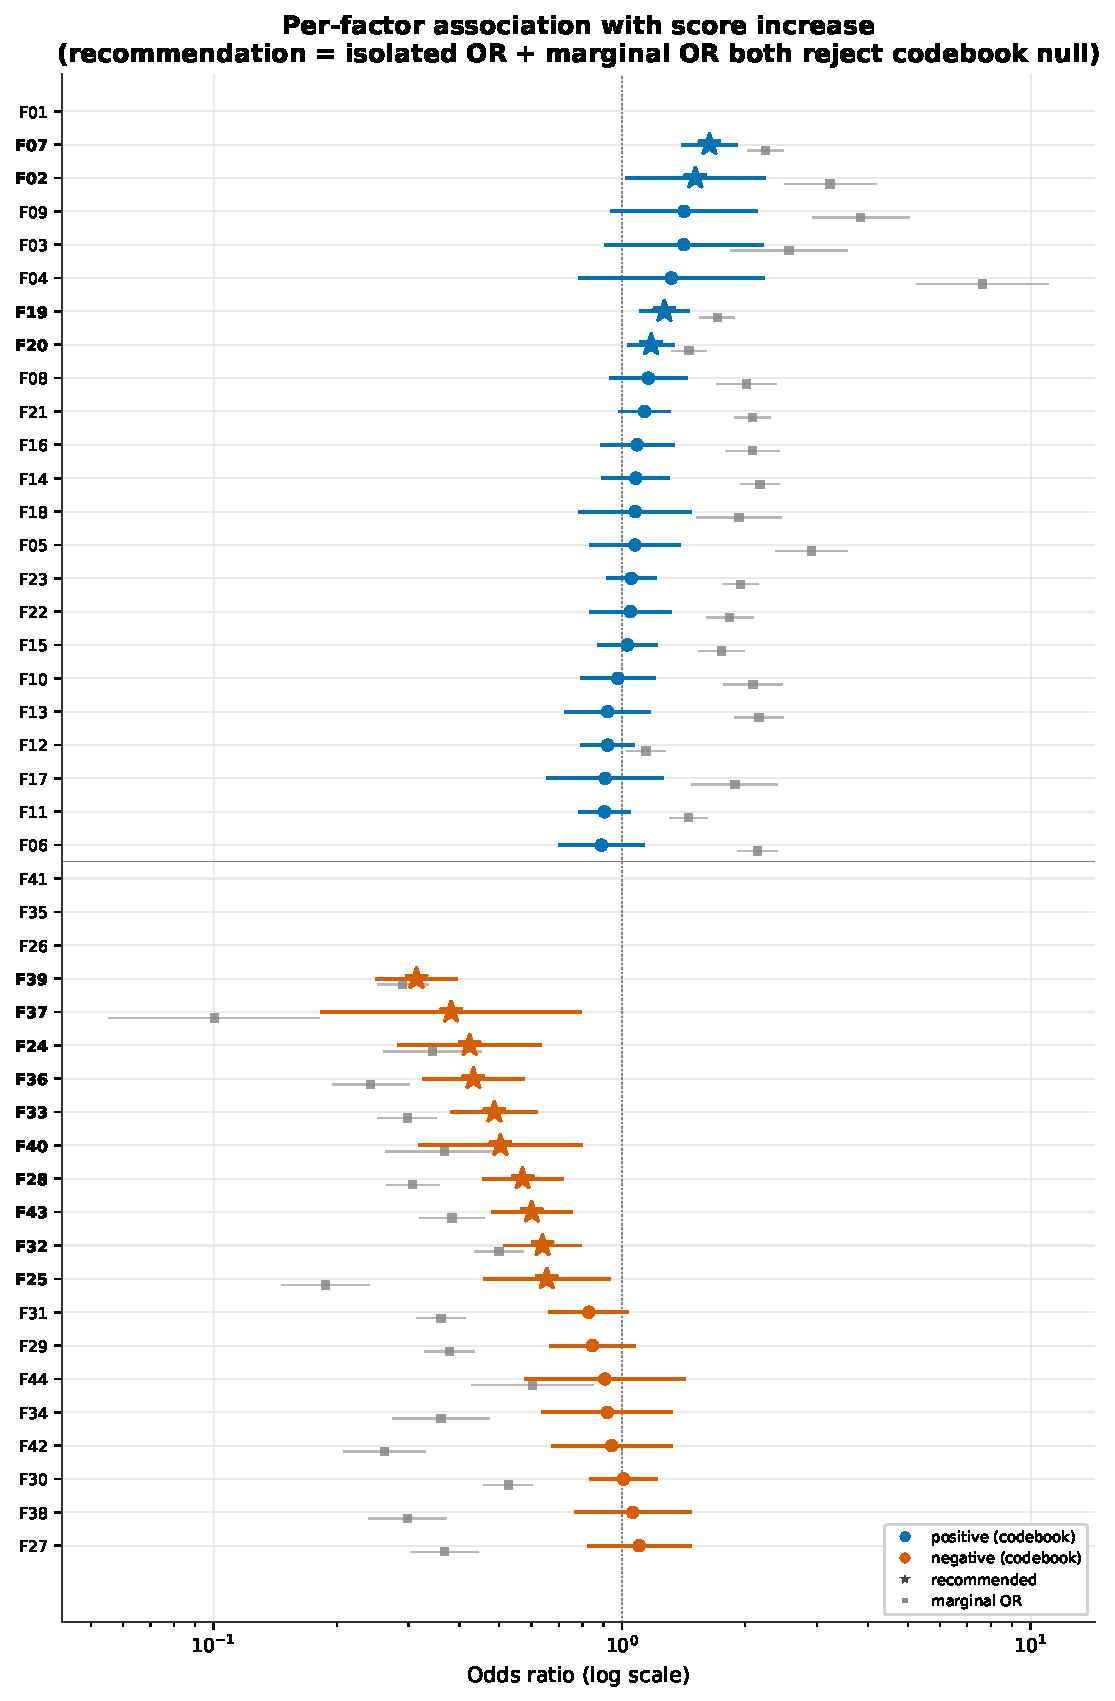
\includegraphics[width=0.68\linewidth]{../../data/results/horizon_inference/figures/forest_recommendation.pdf}
  \caption{\textbf{Per-factor association with score increase, conditional on initial conditions.} Forest plot of the 44 codebook factors, top half (blue) = positive polarity, bottom half (orange) = negative; large markers = polarity-isolated conditional OR (headline joint fit for positives, negatives-only joint fit for negatives), small grey squares = univariate marginal OR, error bars = 95\% cluster-robust CI by paper, $\circ$ = within-codebook-direction, $\star$ = robust association screen met (codebook direction in both marginal and isolated joint fits, both CIs exclude $1$). Four of 23 positive and ten of 21 negative factors qualify. The strongest individual associations are $F_{07}$ baseline completion (OR $= 1.64$ [$1.42$, $1.89$]) on the positive side and $F_{39}$ defensive responses (OR $= 0.31$ [$0.25$, $0.39$]) on the negative side; seven negatives and one positive cross Bonferroni in the headline joint.}
  \label{fig:recforest}
\end{figure}

% ----------------------------------------------------------------------
% Legacy 3.3 (M1-M8 ladder + three triggers) retained for archival
% comparison; replaced by the three-horizon analysis above.
% ----------------------------------------------------------------------
\iffalse
\subsection{[Archived M1-M8 ladder]}\label{res:inference}
% PLACEHOLDER --- one paragraph in a later session.
% Outcome: post-rebuttal score increase (ext_direction == "increase"),
%   binary, ~21\% base rate.
%
% (a) Eight-model paper-clustered logistic ladder (M1--M8).
%   What we did: trained a sequence of paper-clustered logistic models
%     (GroupKFold by paper_key, cluster-robust SEs per CLAUDE.md)
%     predicting score increase. Models progressively add: paper-mean
%     position (M3), full reviewer metadata (M4), Gemini-derived
%     features (M5--M8).
%   What we found: M4 (metadata only) AUC=0.785; M8 (metadata + all
%     Gemini features) AUC=0.791 (+0.006). The largest step is M3
%     (+0.180 AUC), associated with reviewer deviation from paper mean
%     and self-reported confidence (use "associated with" / "tied to",
%     not "driven by", in prose --- predictive language only).
%   Temporal validation (train 2024 -> test 2025) preserves the same
%     model ordering.
%
% (b) Three structural factors as the surviving headline coefficients.
%   (A) Rebuttal effort. Very short rebuttal (~535 words) -> 12-13\%
%       increase; very long (>1574 words) -> 41-42\%. Across all
%       confidence levels.
%   (B) Peer movement. When 76-100\% of co-reviewers also increased,
%       focal reviewer increases at 40-49\% (vs.\ 10-11\% when none
%       moved).
%   (C) Outlier moderated by confidence. Reviewers >=1 sigma below
%       paper mean increase at 49-58\% if low-confidence, but only
%       ~30\% if very high-confidence.
%   Score disagreement per se, number of reviewers, and stance polarity
%     have no effect once the three factors are included
%     (Appendix \ref{app:confidence-triggers}).
%
% Why this framing is honest: because the LLM marginal contribution
%   over metadata is small (3.1(b) and the M8 result here), the linear-
%   model coefficients are interpretable representations of what is
%   recoverable from these features --- not artefacts of overlooked
%   covariates. The predictive ceiling in 3.4 puts this on a firmer
%   footing.
%
% Reference: \Cref{fig:f4-inference}; details in
%   \Cref{app:prediction-comparison,app:confidence-triggers,app:stats}.

[WIP, still old version!!] We trained an eight-model paper-clustered logistic ladder (\Cref{app:prediction-comparison}) predicting the binary outcome ``post-rebuttal score increase'' (\code{ext\_direction == "increase"}), adding feature blocks progressively from initial-score position alone (M1) to all reviewer metadata (M4) to all Gemini-derived features stacked on top of metadata (M8). All cross-validation uses \texttt{GroupKFold} by \code{paper\_key}, since reviews within the same paper are not independent. We report both AUC-ROC and AUPRC because the ${\sim}21\%$ base rate of score increases is moderately imbalanced. Metadata already available on OpenReview (M4: initial-score position, sub-scores, confidence, co-reviewer context, text lengths) reaches AUC = 0.785 and AUPRC = 0.507. Adding all Gemini-extracted features (M8: engagement, tone, sentiment, score offset) lifts AUC to 0.791 and AUPRC to 0.520. Paper-clustered bootstrap (1000 resamples) confirms that the LLM contribution, while small, is statistically real: $\Delta_{\text{AUC}}(\text{M8} - \text{M4}) = +0.006$ [95\% CI: $+0.005$, $+0.007$]. The LLM extracts review signals that are individually informative (M6 alone reaches AUC = 0.689), but those signals are largely redundant with structured metadata. The largest single jump in the ladder is M3 (+0.180 AUC), associated with reviewer deviation from the paper mean and self-reported confidence. Cross-year temporal validation (train 2024, test 2025) preserves the same model ordering.

Within the M4 specification, three structural factors carry the recoverable signal. First, \emph{rebuttal effort}: very short rebuttals (around 535 words) are followed by a 12--13\% score-increase rate, while very long rebuttals (more than \num{1574} words) are followed by 41--42\%. The effort association holds across all confidence levels. Second, \emph{co-reviewer movement}: when 76--100\% of co-reviewers also increased their score, the focal reviewer increased at 40--49\% (vs.\ 10--11\% when no co-reviewers moved). Third, \emph{outlier moderated by confidence}: reviewers at least one standard deviation below the paper mean increased their score at 49--58\% if they were low-confidence, but at only ${\sim}30\%$ if very high-confidence. Score disagreement per se, the number of reviewers, and stance polarity have no association once these three factors are included (\Cref{app:confidence-triggers}). The rebuttal-effort association is a correlation, not a causal effect: papers with more substance to address may both attract longer rebuttals and have more room to improve.

\begin{figure}[t]
  \centering
  \fbox{\parbox[c][5.5cm][c]{0.85\linewidth}{\centering \textit{Figure 4 placeholder
    --- Two-panel composite. (Left) M1-M8 paper-clustered logistic ladder
    with 95\% CIs and per-step incremental gain. (Right) Three-panel
    triggers: rebuttal length quintile, share of co-reviewers who
    increased, and reviewer deviation from paper mean stratified by
    confidence. Sources: data/results/prediction\_comparison/figures/,
    data/results/confidence\_triggers/figures/.}}}
  \caption{\textbf{Controlled regression of score increase: the LLM adds
    little beyond reviewer-level metadata, and three structural factors
    carry the recoverable signal.} (Left) Eight-model paper-clustered
    logistic ladder on \num{73000} reviews, with the +0.006 AUC marginal
    contribution of the full LLM feature set over a metadata-only model
    (M4 vs.\ M8). (Right) Increase rates by rebuttal length, share of
    co-reviewers who also increased, and reviewer deviation from paper
    mean stratified by reviewer confidence.}
  \label{fig:f4-inference}
\end{figure}
\fi

% ----------------------------------------------------------------------
% 3.4 How much does the rebuttal actually move the needle. Operationalises
% the §3.3 inferential model into (a) cascade of predictive performance
% across authoring horizons, (b) out-of-time calibration, (c) scenario
% sensitivities for a representative author. Closes the loop from the
% codebook of §3.2 through the inferential ranking of §3.3 to the
% predicted probability of score increase a writer could read off their
% own draft.
% ----------------------------------------------------------------------
\subsection{How much does an author's rebuttal move the needle}\label{sec:rebuttal-impact}

\Cref{sec:horizons} identifies which behaviors are conditionally associated with success. Three questions an author would actually ask follow: how much of the post-rebuttal outcome is locked in by the situation versus movable by what they write, how trustworthy are the model's predicted probabilities on out-of-time data, and what does adding or removing recommended behaviors do to the predicted probability for a representative author? We answer each with the same rebuttal-content logistic of \Cref{sec:horizons}, sliced three different ways. \Cref{app:horizons} carries the cohort definition, the full feature catalogue at each horizon (pre-rebuttal, rebuttal-content, post-discussion), the evaluation protocol (temporal split and paper-clustered $\texttt{GroupKFold}(5)$), and the leakage audit.

The pre-rebuttal logistic, fit on structural confounders, review-text features, and Gemini text-derived signals visible before the author has written anything, already reaches $\auc = 0.744$ [$0.71$, $0.77$] / $\auprc = 0.722$ [$0.68$, $0.76$] on the temporal test (\Cref{fig:horizons}). A substantial part of the score-revision signal is therefore set by initial conditions, namely the focal reviewer's deviation from the paper's initial mean, their initial-score position, and the LLM-decoded text-vs-score offset of \Cref{res:instrument}. Adding the rebuttal-text aggregates and 44 factor indicators lifts both metrics to $\auc = 0.801$ [$0.78$, $0.83$] and $\auprc = 0.779$ [$0.74$, $0.81$], a temporal-split gain of $\Delta\auc = +0.057$ and $\Delta\auprc = +0.057$ that replicates under cross-validation as $\Delta\auc = +0.068$ ($0.778 \pm 0.006 \to 0.846 \pm 0.010$). The two metrics agree on the magnitude of the rebuttal-content lift, which is what we would expect at the cohort's base rate of $44.4\%$ (no class imbalance distortion). Adding co-reviewer-movement and thread-depth aggregates at the post-discussion horizon adds little on top ($\Delta\auc = +0.005$ on the temporal split, $+0.009$ in cross-validation), and the single feature \code{co\_reviewer\_post\_change\_mean} reaches $\auc \approx 0.65$ on its own, so the post-discussion lift is largely redundant with the rebuttal-content features. \emph{Most of the recoverable signal is locked in before the author writes anything, and the rebuttal contributes a real but bounded $+0.06$ to $+0.07$ AUC of incremental signal at rebuttal-content.} A random forest on the same features at every horizon never exceeds the logistic by more than $0.01$ AUC (RF rebuttal-content $\auc = 0.767$ vs logistic $0.801$ on the temporal split, $0.834 \pm 0.009$ vs $0.846 \pm 0.010$ under cross-validation), so the linear model of \Cref{sec:horizons} reaches the predictive ceiling reachable from these features and the inferential ORs of \Cref{fig:recforest} are not artefacts of an under-fit linear approximation.

\begin{figure}[!htb]
  \centering
  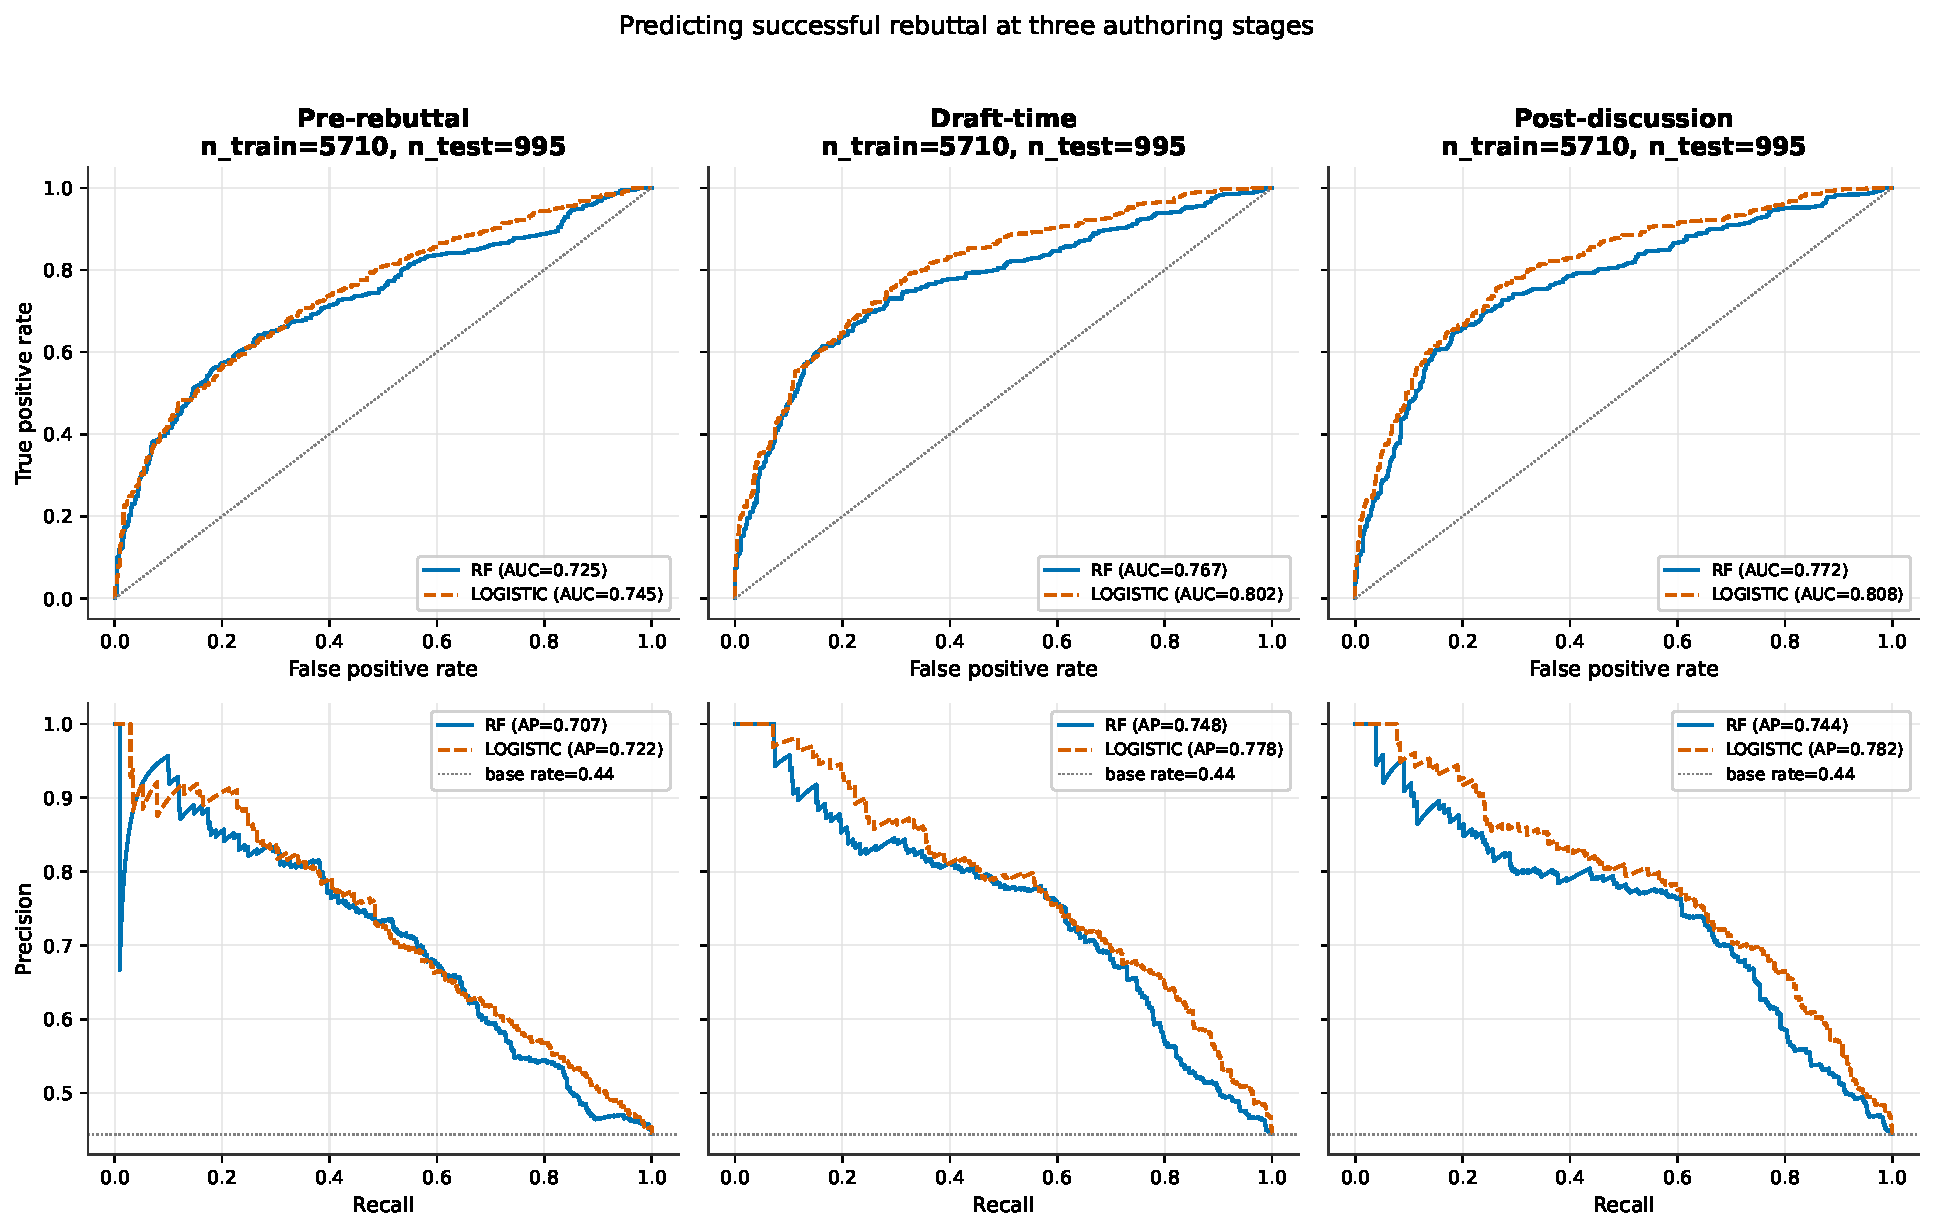
\includegraphics[width=0.85\linewidth]{../../data/results/rebuttal_rf_prediction/figures/figure_horizons.pdf}
  \caption{\textbf{Cascade of predictive performance across authoring horizons.} ROC (top) and precision-recall (bottom) curves for random forest (solid blue) and L2-regularised logistic (dashed orange) on the temporal split (train ICLR 2024, $n=5{,}710$; test ICLR 2025, $n=995$). Pre-rebuttal features alone reach $\auc = 0.744$. Adding rebuttal-content features at rebuttal-content lifts $\auc$ by $+0.057$. Co-reviewer movement at the post-discussion horizon adds $+0.005$ on top, mostly redundant with the rebuttal content. Across all three horizons the random forest never exceeds the logistic by more than $0.01$ AUC.}
  \label{fig:horizons}
\end{figure}

Out-of-time calibration (\Cref{fig:calibration}) is reliable at the extremes. The top decile predicts $0.94$ against an observed $0.89$, and the bottom decile predicts $0.05$ against an observed $0.14$. Two middle deciles over-predict by up to $0.16$ (the worst is the predicted-$0.65$ bin at $49\%$ observed). The rank ordering carries the load across the full range, but the absolute probability scale is reliable mainly at the extremes, so a fixed-threshold readout under-uses the information the model carries. Threshold metrics at $p = 0.5$ are reported in \Cref{tab:threshold-metrics} and \Cref{app:horizons} for context only ($72.6\%$ accuracy, $F_1 = 0.71$ on the 995-row temporal test against a $44.4\%$ base rate, and $77.1\%$ / $F_1 = 0.75$ under paper-clustered $\texttt{GroupKFold}(5)$ on the full $n = 6{,}705$ pool). The 2025 evaluation slice is the stratified \Cref{res:rebuttal-categories} (Test 1) sample rather than a representative draw, so the per-bin observed rates are themselves noisy and the calibration plot reads as a sanity check on the predictive horizon, not as the basis for an interventional prescription on a specific draft.

\begin{figure}[!htb]
  \centering
  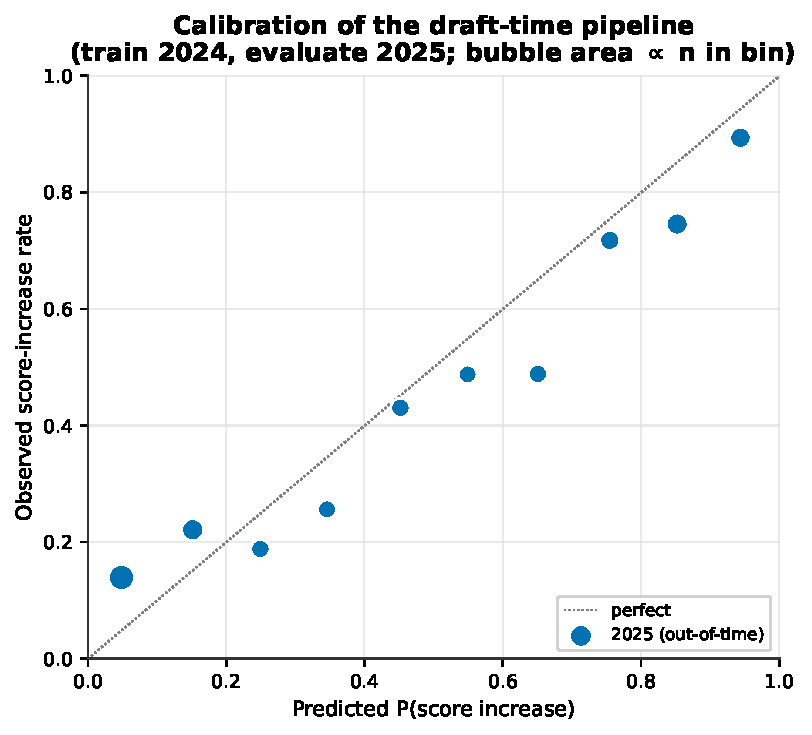
\includegraphics[width=0.55\linewidth]{../../data/results/horizon_inference/figures/calibration_temporal.pdf}
  \caption{\textbf{Out-of-time calibration of the rebuttal-content pipeline.} Train ICLR 2024 logistic; predict on the ICLR 2025 stratified slice ($n = 995$); bin by predicted probability into deciles. Bubble area is proportional to bin sample size. Top and bottom deciles track the diagonal within ${\sim}0.05$ ($0.94 \to 0.89$ and $0.05 \to 0.14$ respectively), while two middle deciles (predicted $\sim 0.65$ and $\sim 0.85$) over-predict by up to $0.16$. The 2025 slice is a stratified rather than representative sample, so the per-bin observed rates are themselves noisy.}
  \label{fig:calibration}
\end{figure}

Holding a 2024-median author profile fixed (median initial score, median paper mean, neutral confidence, neutral Gemini offset), the model's predicted probability of score increase is $0.22$ for a rebuttal with no qualifying factors present, $0.32$ for a rebuttal with $F_{07}$ baseline completion present, $0.47$ for one with the top-3 qualifying positives ($F_{07}$, $F_{02}$, $F_{19}$) present, and $0.53$ for one with all four ($F_{07}$, $F_{02}$, $F_{19}$, $F_{20}$) (\Cref{tab:scenarios}). A rebuttal that exhibits the top-3 qualifying negatives ($F_{39}$, $F_{37}$, $F_{24}$) alongside all four qualifying positives sits at $0.09$, and one that exhibits only the negatives sits at $0.02$. The directional asymmetry is informative: rebuttals without the top qualifying negatives carry predicted probabilities comparable to rebuttals with the top qualifying positives. These probabilities are conditional under the observational model, not interventional estimates. An interventional version would require randomised assignment of factor inclusion across rebuttals, which our design cannot deliver. The scenario probabilities also inherit the middle-decile miscalibration above. With those caveats, the magnitudes give a sense of the rebuttal-attributable lever associated with each configuration.

\begin{table}[t]
  \centering
  \caption{Predicted score-increase probability under the rebuttal-content logistic for a 2024-median author profile whose rebuttal already exhibits the listed factors. The numbers are conditional probabilities under the observational model, not interventional estimates. ``Top-$k$ qualifying'' refers to the $k$ factors with the largest isolated odds ratio in the codebook direction among those that meet the asymmetric association screen (\Cref{fig:recforest}). Probabilities read off the same rebuttal-content logistic used in \Cref{sec:horizons}.}
  \label{tab:scenarios}
  \small
  \begin{tabular}{lr}
    \toprule
    Rebuttal configuration (factors observed to be present) & $P(\text{score increase})$ \\
    \midrule
    Median author profile, no qualifying factors                                       & $0.22$ \\
    With $F_{07}$ baseline completion present                                          & $0.32$ \\
    With the top-3 qualifying positive factors present                                 & $0.47$ \\
    With all four qualifying positive factors present                                  & $0.53$ \\
    With all four positives \emph{and} top-3 negatives present                         & $0.09$ \\
    With top-3 qualifying negative factors only (no positives)                         & $0.02$ \\
    \bottomrule
  \end{tabular}
\end{table}

The pipeline of \Cref{res:instrument} (Gemini score-decoder), \Cref{res:rebuttal-categories} (44-factor classifier), and the rebuttal-content logistic of \Cref{sec:horizons} together map a rebuttal draft plus the publicly visible reviewer/paper metadata to a predicted probability of score increase. The qualifying-factor list of \Cref{fig:recforest} and the scenario sensitivities of \Cref{tab:scenarios} are the paper's contribution at the actionable end: a robust association screen over which behaviors are most strongly tied to a score increase, and an order-of-magnitude sense of how much adding or removing them shifts the model's predicted probability for a representative author. The predictions are correlational summaries of observed outcomes, the LLM components inherit the failure modes of \Cref{res:instrument,res:rebuttal-categories}, the 2025 evaluation uses a stratified slice rather than a representative one, and the calibration is reliable only at the extremes. Reading the screen as an interventional recipe (``insert these factors into your draft and the score will rise by this much'') is not warranted by the evidence.

% ======================================================================
% 4. DISCUSSION
% ======================================================================
\section{Discussion}\label{sec:discussion}

\paragraph{Synthesis.} The clearest reading of our results is that most of what predicts a post-rebuttal score increase is set before the author writes a word. Pre-rebuttal features alone reach $\auc = 0.744$, and the rebuttal-content horizon adds only $+0.057$. Within that bounded contribution, two things matter. The 44-factor content codebook does most of the work, with a small number of factors meeting our asymmetric robust-association screen ($F_{07}$ baseline completion, $F_{39}$ defensive responses, and a handful of others) and the LLM-detected text-vs-score offset surviving as an independent but modest contributor. And the rebuttal-content lift is concentrated where the structural lever is weakest, namely near-paper-mean reviewers, where the cascade gain is $+0.092$ AUC versus $+0.056$ for above-mean reviewers. The picture is neither fully predetermined nor primarily rhetorical. Reviewer movability is structured before the rebuttal arrives, but the rebuttal still carries a real, bounded slice of predictability, and that slice is dominated by content moves rather than tone or rhetorical posture.

\paragraph{Why the LLM-text signal is bounded.} The Gemini score-decoder is a usable instrument, with a monotonic post-rebuttal increase rate across the offset gradient ($8\%$ to $19\%$ to $32\%$) that a constant-mode predictor cannot produce. But once the 44 factor indicators are in the regression, the offset's marginal contribution shrinks to OR $= 1.16$. We read this as the codebook capturing the operationalisable end of the same text Gemini reads, with the offset retaining a residual signal that mediation analyses suggest is largely independent of stance and engagement. The score-vs-confidence asymmetry is the natural companion to this finding. The score is anchored to the substantive critique by argumentative coherence, so LLMs decode it moderately well from text alone (Spearman $\rho = 0.40$). The reviewer's self-reported confidence has no textual referent, the LLM collapses onto the modal value $4$, and the asymmetry constrains what self-reported confidence can carry, since whatever it tracks is mostly not in the words the reviewer wrote.

\paragraph{Implications for authors and for venues.} For authors, the recommendation screen is a robust association list and not a causal recipe. Avoiding the qualifying negatives moves the predicted probability of an increase comparably to adding the qualifying positives, so defensiveness is more costly than baseline completion is rewarding. For venues, the rebuttal mechanism resolves a measurable share of the score-disagreement noise that reviewing produces, but not all of it. The top-decile and bottom-decile observed-success rates of $0.89$ and $0.14$ show that the model's rank-ordering is reliable across the full range, while two middle deciles miscalibrate by up to $0.16$, so any threshold-based readout under-uses the information the model carries. LLMs are useful as text-decoding instruments and as factor classifiers under outcome-blinded protocols, not as adjudicators that replace reviewer scoring.

\paragraph{Limitations.} The corpus is ICLR 2024 and 2025 only and the rating scale is ordinal with uneven steps, both of which limit cross-venue and cross-time portability. The 2025 cohort is a stratified $1{,}000$-pair sample rather than a representative random draw, after a budgeted full-2025 batch failed at submission and was not re-attempted within budget. All statistical language is correlational. We use paper-clustered standard errors, but there is no causal identification, and observed associations may reflect unmeasured paper-level confounds. The rebuttal-content horizon is observationally defined, since factor indicators are extracted from the resolved thread including reviewer follow-ups, so per-factor odds ratios should be read as properties of the resolved interaction rather than as guarantees about the author's first-shot draft. Within-rebuttal multicollinearity between positive and negative factors required the asymmetric polarity screen, so individual joint coefficients should be interpreted alongside the marginal and polarity-isolated refits in \Cref{app:horizons}. The ICLR 2025 portion of our corpus overlaps with the randomised LLM-feedback intervention of Thakkar et al.~\cite{thakkar}, in which roughly 27\% of treated reviewers updated their reviews based on LLM feedback. We did not exclude treatment-arm reviews because the assignment indicators are not public. Because the intervention was randomised at the reviewer level, any effect on our estimates should average out across the corpus rather than bias them in a known direction. The ICLR 2024 cohort, used as the temporal training year for all year-train-on-2024 evaluations, predates the intervention and is uncontaminated. If treatment indicators become available, the analyses would be straightforwardly recomputable on the untreated subset.

\paragraph{Future work.} Three directions follow. First, cross-venue replication on NeurIPS, ICML, and less-anonymised conferences, where the base rate of post-rebuttal change and the structural confounders may shift. Second, prospective intervention studies, where the recommendation screen's correlational claims are tested against actual draft-level edits, since the gap between association and causation is the most consequential limitation of the present analysis. Third, a draft-only re-classification of the 44 factors on first-shot rebuttal text (excluding reviewer follow-ups), which would isolate author-controllable factors from emergent ones and sharpen the per-factor odds ratios for use in writing guidance.

% ======================================================================
% 5. REFERENCES (bibliography)
% ======================================================================
% TEMPORARY: \nocite{*} forces all references.bib entries into the printed
% bibliography while the main-text prose has no real \cite{...} calls yet.
% Remove once Introduction/Discussion drafts cite each reference explicitly.
\nocite{*}
\bibliography{references}

% ======================================================================
% 6. APPENDIX / METHODS  (the "blueprint" container)
% ======================================================================
\clearpage
\appendix

\section{Methods and supplementary materials}\label{app:methods}
% Umbrella section. Each \subsection below is a methodological block
% referenced from the main text. Subsection bodies are placeholders;
% content sources are listed in comments so prose can be drafted in a
% follow-up session by salvaging from main.tex and the docs/methodology/
% files.

\subsection{Dataset}\label{app:dataset}

We collected all publicly visible submissions, reviews, decisions, and discussion data from four years of ICLR (2023--2026) via the OpenReview API on the following dates: ICLR 2023--2024 on November 3, 2025, ICLR 2025 on January 21, 2026, and ICLR 2026 on March 31, 2026. The latest discussion activity recorded is May 2, 2025 for ICLR 2025 and March 28, 2026 for ICLR 2026. Table~\ref{tab:dataset-appendix} provides the per-year composition.

\begin{table}[htbp]
  \centering
  \caption{Extended dataset composition. Message counts reflect individual posts. Engagement rates count distinct participant-paper events. Acceptance rates differ slightly from PaperCopilot for 2023 (footnote $d$) and for 2024--2025 (footnote $e$); for 2026, rates match exactly.}
  \label{tab:dataset-appendix}
  \small
  \begin{tabular}{lrrrrr}
    \toprule
    & \textbf{2023} & \textbf{2024} & \textbf{2025} & \textbf{2026} & \textbf{Total} \\
    \midrule
    Papers (total)                & \num{3793}  & \num{7404}  & \num{11672} & \num{19814} & \num{42683}  \\
    \quad with reviews            & \num{3793}  & \num{7262}  & \num{11520} & \num{19474} & \num{42049}  \\
    \quad without reviews         & 0           & 142         & 152         & 340         & 634          \\
    Reviews                       & \num{14339} & \num{28028} & \num{46748} & \num{75859} & \num{164974} \\
    Reviews per paper             & 3.8         & 3.9         & 4.1         & 3.9         & 3.9          \\
    \midrule
    Discussion messages           & \num{36875} & \num{70624} & \num{149221}& \num{180144}& \num{436864} \\
    \quad Author messages         & \num{30189} & \num{56082} & \num{115034}& \num{159454}& \num{360759} \\
    \quad Reviewer messages       & \num{6376}  & \num{14016} & \num{32938} & \num{19559} & \num{72889}  \\
    \quad AC/PC messages          & 310         & 526         & \num{1235}  & \num{1131}  & \num{3202}   \\
    Author response rate$^a$      & 88.7\%      & 80.1\%      & 74.6\%      & 74.0\%      &              \\
    Reviewer follow-up rate$^b$   & --          & 17.5\%      & 17.7\%      & 12.2\%$^c$  &              \\
    \midrule
    Acceptance rate (ours)        & 41.5\%$^d$  & 30.5\%      & 31.7\%      & 27.0\%      &              \\
    Acceptance rate (PaperCopilot)& 31.8\%      & 31.0\%      & 32.1\%      & 27.0\%      &              \\
    Rating scale                  & \multicolumn{3}{c}{$\{1, 3, 5, 6, 8, 10\}$} & $\{0, 2, 4, 6, 8, 10\}$ & \\
    API version                   & v1          & \multicolumn{3}{c}{v2} &              \\
    \bottomrule
  \end{tabular}
\end{table}

\noindent\footnotesize
$^a$ Fraction of papers with at least one author comment.
$^b$ Fraction of reviews where the reviewer posted at least one follow-up comment. Not available for 2023 (API v1 does not reliably distinguish reviewer follow-ups from initial reviews).
$^c$ ICLR 2026 data was collected March 31, 2026. The low reviewer follow-up rate likely reflects incomplete discussion data, as the latest recorded follow-up is March 28, 2026.
$^d$ Our 2023 acceptance rate (41.5\%) differs from PaperCopilot (31.8\%) because our dataset is missing ${\sim}\num{1162}$ withdrawn or desk-rejected papers (see below). PaperCopilot computes acceptance over all \num{4955} submissions.\\
$^e$ The 0.4 to 0.5 percentage-point gap for 2024 and 2025 likely reflects papers that were accepted and then later withdrawn. We classify these by final OpenReview status (Withdrawn), while PaperCopilot may count by acceptance decision.
\normalsize

\paragraph{ICLR 2023: missing withdrawn and desk-rejected papers.}
ICLR 2023 data was accessed through OpenReview API v1. Withdrawn and desk-rejected papers are no longer publicly accessible through this API. Our ICLR 2023 subset therefore contains only \num{3793} papers, whereas PaperCopilot reports \num{4955} total submissions for ICLR 2023~\cite{papercopilot}. The roughly \num{1162} missing papers are most likely a mix of withdrawn submissions and desk rejections. All \num{3793} papers in our 2023 dataset have reviews, consistent with the missing papers being those removed before or during the review process. For 2024 to 2026, our paper counts match PaperCopilot exactly.

\paragraph{ICLR 2026: rating scale change.}
All four years use a six-point discrete scale with the same descriptive labels (``strong reject'', ``reject, not good enough'', ``marginally below the acceptance threshold'', ``marginally above the acceptance threshold'', ``accept, good paper'', ``strong accept, should be highlighted at the conference''). The numeric values changed in 2026 from $\{1, 3, 5, 6, 8, 10\}$ (used in 2023 to 2025) to $\{0, 2, 4, 6, 8, 10\}$. The lowest score moved from 1 to 0, and the below-threshold scores shifted from $\{3, 5\}$ to $\{2, 4\}$, widening the gap between weak reject (2) and weak accept (4) compared to the previous scale where 5 and 6 were adjacent. Cross-year score comparisons normalise to ordinal positions (step 1 through step 6) rather than raw values, or exclude 2026 when the scale difference is material.

\paragraph{ICLR 2026: no Spotlight tier in the data.}
Our ICLR 2026 data contains no papers with a Spotlight decision. In 2023 to 2025, Spotlight served as an intermediate acceptance tier between Oral and Poster. ICLR 2026 papers are classified only as Oral (\num{224}), Poster (\num{5132}), Rejected (\num{9313}), or Withdrawn (\num{5145}). We cannot determine from our data whether ICLR 2026 formally eliminated the Spotlight category or whether Spotlight designations had not yet been publicly announced at the time of data collection (March 31, 2026). Cross-year comparisons by decision tier account for this difference.

\subsection{Normalization pipeline}\label{app:normalization}

The OpenReview platform underwent significant structural changes between 2023 (API v1) and 2024 to 2026 (API v2), and ICLR itself modified its review form across years. Table~\ref{tab:format-differences} summarises the key differences that our normalisation pipeline reconciles.

\begin{table}[htbp]
  \centering
  \caption{Format differences across ICLR years. The 2023 format (API v1) differs substantially from 2024 to 2026 (API v2). These differences make naive cross-year analysis fail silently without a normalisation layer.}
  \label{tab:format-differences}
  \small
  \begin{tabular}{p{3.5cm} p{5cm} p{5cm}}
    \toprule
    \textbf{Feature} & \textbf{2023} & \textbf{2024 to 2026} \\
    \midrule
    API version
      & v1
      & v2 \\
    Invitation field
      & \code{invitation} (single string)
      & \code{invitations} (array of strings) \\
    Content wrapping
      & Direct values (e.g., \code{"rating": "6: ..."})
      & Wrapped values (e.g., \code{"rating": \{"value": "6: ..."\}}) \\
    Rating field name
      & \code{recommendation}
      & \code{rating} \\
    Summary field
      & \code{summary\_of\_the\_paper}
      & \code{summary} \\
    Strengths/weaknesses
      & Combined: \code{strength\_and\_weaknesses}
      & Separate: \code{strengths}, \code{weaknesses} \\
    Decision encoding
      & Venue-text (e.g., ``notable top 5\%'' to Oral, ``Submitted to ICLR 2023'' to Rejected)
      & Explicit decision notes \\
    Withdrawn tracking
      & Not explicitly recorded
      & Explicit Withdrawn status \\
    Primary area field
      & \code{Please\_choose\_the\_closest\_area\ldots}
      & \code{primary\_area} \\
    \bottomrule
  \end{tabular}
\end{table}

These differences mean that naive cross-year analysis would fail silently. For example, reading \code{paper["content"]["rating"]} across all years would miss ICLR 2023 data entirely (where the field is called \code{recommendation}), or return wrapped dictionaries instead of values for 2024+ data.

We implemented a normalisation pipeline using the template method pattern. A \code{BaseConverter} abstract class defines shared conversion logic (value unwrapping, rating extraction, participant classification, decision normalisation), while per-conference subclasses handle year-specific field mappings. The pipeline auto-detects the appropriate converter based on the source filename. Participant classification assigns each discussion comment to a type (author, reviewer, area chair, program chair) based on signature patterns in the OpenReview data, enabling separate analysis of author rebuttals, reviewer follow-ups, and editorial interventions. Output files are written as JSON with a manifest recording conversion metadata (schema version, source file, paper/review/comment counts, conversion date). All \num{164974} reviews in the normalised output have complete rating, summary, strengths, and weaknesses fields. This reflects OpenReview's requirement that reviewers fill in these fields when submitting a review.

\subsection{External ground truth reconciliation}\label{app:ext-gt}

We use the reviewer-level before- and after-rebuttal scores published by Kargaran et al.~\cite{kargaran} as ground truth for validating both score predictions and score-change detection. This subsection documents the reconciliation between their dataset and ours.

\begin{table}[htbp]
  \centering
  \caption{Reconciliation between our OpenReview dataset and the external ground truth from Kargaran et al. ``With scores'' indicates papers where reviewer-level before/after ratings are available. ``Empty'' papers appear in the external dataset with a title but no reviewer-level data.}
  \label{tab:external-gt}
  \small
  \begin{tabular}{lrrrr}
    \toprule
    & \multicolumn{2}{c}{\textbf{ICLR 2024}} & \multicolumn{2}{c}{\textbf{ICLR 2025}} \\
    \cmidrule(lr){2-3} \cmidrule(lr){4-5}
    & Papers & Reviews & Papers & Reviews \\
    \midrule
    Our dataset (all)              & \num{7404}  & \num{28028}  & \num{11672} & \num{46748}  \\
    \quad with reviews             & \num{7262}  & \num{28028}  & \num{11520} & \num{46748}  \\
    External GT (total entries)    & \num{7407}  &              & \num{11677} &              \\
    \quad with reviewer scores     & \num{6973}  & \num{26878}  & \num{11431} & \num{46353}  \\
    \quad empty (no reviewer data) & 434         & --           & 246         & --           \\
    \midrule
    Matched (reviews in both)      &             & \num{26878}  &             & \num{46353}  \\
    Only in our data               &             & \num{1150}   &             & 395          \\
    \bottomrule
  \end{tabular}
\end{table}

\paragraph{Papers without reviewer scores in the external dataset.}
The external dataset contains entries for \num{7407} ICLR 2024 papers and \num{11677} ICLR 2025 papers. However, 434 (2024) and 246 (2025) of these entries have no reviewer-level score data: the paper title and tracing score are present, but the review dictionary is empty. These 680 empty entries fall into two distinct categories.

\textit{Case 1: papers with reviews that the external scraper missed (379 papers).} Of the 680 empty entries, 289 in 2024 and 90 in 2025 correspond to papers that do have reviews in our dataset and on the OpenReview website. These 379 papers account for \num{1545} reviews for which we have the final score and Gemini predictions but no before/after ground truth. We verified a sample by re-querying the OpenReview API (April 2026): all sampled papers have full review data publicly accessible, so the missing entries reflect coverage of the external before/after scrape rather than the underlying OpenReview records. These papers do not differ systematically from covered papers on decision distribution (54.8\% Rejected vs.\ 47.3\%), mean rating (5.15 vs.\ 5.14), review dates, or topic areas.

\textit{Case 2: withdrawn or desk-rejected papers with no reviews anywhere (301 papers).} The remaining 145 (2024) and 156 (2025) empty entries correspond to papers that also have zero reviews in our data and on the OpenReview website. Neither dataset has review data for them because no reviews were ever written.

\paragraph{OpenReview ratings reflect post-rebuttal scores.}
A critical point for our validation methodology: the rating returned by the OpenReview API reflects the reviewer's final (post-rebuttal) score, not the initial score. We confirmed this by comparing the OpenReview rating against the after-rebuttal score from the external ground truth: 100\% exact match across all \num{26878} matched reviews in ICLR 2024 and all \num{46353} matched reviews in ICLR 2025. This means that comparing LLM score predictions against OpenReview ratings would conflate two effects: prediction error and rebuttal-induced score changes. Since our LLM predicts scores from the original review text (written before any rebuttal), the appropriate comparison is against the initial pre-rebuttal score from the external dataset. All prediction-accuracy figures in this paper use the initial pre-rebuttal score as ground truth.

\paragraph{Review-count discrepancies.}
For ICLR 2024, our dataset contains \num{28028} reviews while the external dataset contains \num{26878} reviewer-level records. The difference of \num{1150} reviews comes entirely from the 289 papers with empty review records in the external data. Within papers that both datasets cover, the reviewer-level match is exact. For ICLR 2025, the reviewer-level match is also exact: all \num{46353} reviewer records in the external dataset are matched in our data.

\subsection{Gemini score-prediction protocol}\label{app:gemini-pred}

\paragraph{Task.}
We tested whether Gemini Flash 3 can infer reviewer scores from review text alone, without access to any numeric rating fields. We submitted all ICLR 2024 and 2025 reviews to the Gemini Batch API (model: \code{gemini-3-flash-preview}) with a structured prompt requesting per-reviewer inferred scores on the ICLR discrete scale $\{1, 3, 5, 6, 8, 10\}$, along with confidence, sentiment, and engagement-quality ratings. Temperature was set to 0.0 for deterministic output. The full prompt is reproduced in \Cref{app:prompts}.

\paragraph{Score-field stripping.}
Before sending reviews to the LLM, we removed all numeric scoring fields to prevent the model from reading the score rather than inferring it from the review text. The strip set covers, across all years: \code{soundness}, \code{presentation}, \code{contribution}, \code{rating}, \code{recommendation}, and \code{confidence} (the reviewer's self-reported confidence on a 1--5 scale). For ICLR 2023 reviews, the strip set additionally covers the year-specific sub-scores: \code{correctness}, \code{technical\_novelty\_and\_significance}, \code{empirical\_novelty\_and\_significance}, and \code{clarity,\_quality,\_novelty\_and\_reproducibility}. Matching is case- and space-insensitive (e.g., ``Confidence'' and \code{confidence} both match) to handle formatting variations across years. After stripping, the fields remaining in the input dict for an ICLR 2024 to 2025 review are the four free-text fields written by the reviewer (\code{summary}, \code{strengths}, \code{weaknesses}, \code{questions}) plus the boolean ethics flag (\code{flag\_for\_ethics\_review}). The boolean flag is binary metadata that cannot leak the score. The implementation is in \code{src/experiment/batch\_utils.py:remove\_score\_fields}.

\paragraph{Batch processing.}
ICLR 2024 was processed in 25 chunks (February to March 2026), ICLR 2023 in 13 chunks (March 14 to 15, 2026), and ICLR 2025 in 12 chunks (March 24, 2026). Papers without reviews were excluded: 142 in ICLR 2024, 152 in ICLR 2025. Neither the batch input files nor the output files contain model metadata. The model version was confirmed via the batch tracker, which records the runtime environment variable at submission time.

\paragraph{Validation against the initial pre-rebuttal score.}
We validated predictions against the initial pre-rebuttal scores from the external ground truth (\Cref{app:ext-gt}), not the final post-rebuttal scores visible on OpenReview. Combined across ICLR 2024 and 2025 ($n = \num{73000}$): exact match 40.7\%, within-one-step 87.6\%, Spearman $\rho = 0.403$. By year: ICLR 2024 reaches 36.9\% / 81.2\% / $\rho = 0.330$ ($n = \num{26805}$). ICLR 2025 reaches 42.9\% / 91.2\% / $\rho = 0.457$ ($n = \num{46195}$). We report Spearman $\rho$ rather than Pearson $r$ because the ICLR scale has uneven step sizes (\{1, 3, 5, 6, 8, 10\} with gaps 2, 2, 1, 2, 2). Pearson's magnitude depends on the (arbitrary) numeric spacing of the scale, while Spearman, being rank-based, is invariant to it. Source figures: \code{data/results/gemini\_prediction/figures/}.

\paragraph{Offset operationalisation.}
The text-vs-score offset used throughout \Cref{res:instrument,sec:horizons,sec:rebuttal-impact} and \Cref{app:text-score-gap} is computed as a difference of \emph{step positions} on the six-point ICLR ladder, not a difference of raw rating points. Concretely, both the Gemini-decoded score and the assigned initial score are first mapped through the position table $\{1{:}0,\, 3{:}1,\, 5{:}2,\, 6{:}3,\, 8{:}4,\, 10{:}5\}$ and the offset is the difference of indices. Two reviewers who are ``one step apart'' on the ladder always have $|\code{offset}| = 1$ regardless of where on the scale they sit, so the $5 \to 6$ adjacent pair is treated identically to the $8 \to 10$ adjacent pair. Reading the offset in raw rating points would conflate the $5{-}6$ jump (one ladder step but one raw point) with the $6{-}8$ jump (also one ladder step but two raw points) and bias the regression coefficients accordingly. The mean offset of $+0.14$ and standard deviation of $1.02$ reported throughout the paper are therefore in step units. The funnel buckets of \Cref{fig:f2-funnel} collapse the offset to its sign only (\code{under} for $\code{offset} < 0$, \code{match} for $\code{offset} = 0$, \code{over} for $\code{offset} > 0$); the regressions of \Cref{sec:horizons,sec:rebuttal-impact} use the integer step difference standardised by year-pooled mean and standard deviation. Implementation: \code{src/analyze/prediction\_comparison.py:62--214}.

\paragraph{Distributional fidelity, not raw accuracy, is the right yardstick.}
The within-one-step accuracy of 87.6\% is not load-bearing evidence on its own: a constant predictor that always emits the modal score 5 reaches 88.8\% within one step on the same data, simply because the assigned scores cluster around 5--6. What that constant predictor \emph{cannot} do, and what the analyses in \Cref{res:instrument} require, is produce a per-review prediction that varies with the input text. Two pieces of evidence speak directly to per-review informativeness. First, Gemini's prediction distribution spans the ICLR scale and roughly tracks the assigned distribution: 0.4\% / 19\% / 46\% / 27\% / 7\% / 0.0\% on \{1, 3, 5, 6, 8, 10\} for predictions vs.\ 2.4\% / 30\% / 35\% / 24\% / 9\% / 0.3\% for assigned scores. Second, the LLM-decoded-minus-assigned offset predicts post-rebuttal score-increase rates of 8.3\% / 19.2\% / 31.9\% across the three offset bins (\Cref{app:text-score-gap}), which is information no constant predictor can encode because its offset would be a deterministic function of the assigned score alone.

\paragraph{Inferred reviewer confidence is uninformative.}
The same prompt requested a per-reviewer inferred confidence on the same 1--5 scale the reviewer self-reports (and which we stripped from the input). Unlike the score, the confidence channel \emph{is} essentially collapsed onto a single value: across \num{74545} reviews, Gemini predicts confidence 4 in 80\% of cases against a true rate of 47\%, predicts 3 in only 11\% (vs.\ 33\% true), and predicts 5 in 7\% (vs.\ 13\% true). Spearman rank correlation against the held-out self-reported confidence is $\rho = 0.29$ for ICLR 2024 and $\rho = 0.06$ for ICLR 2025 (combined $\rho = 0.18$). The headline accuracy figures (48.2\% exact, 91.1\% within one step) sit close to a constant-mode predictor of confidence (47.2\% / 92.8\%) and reflect the same cluster-on-the-mode behavior, not text-conditioned per-review signal. Because the predictions are near-constant, no analog to the offset funnel can be constructed, so the same downstream test that validated the score channel cannot rescue confidence. We therefore do not use the inferred reviewer confidence as a feature anywhere in the paper.

\subsection{Score-change detection: Gemini vs.\ regex validation}\label{app:score-change}

We developed a two-stage pipeline to detect whether reviewers changed their scores after author rebuttals. OpenReview records only final scores, not score histories, so changes must be inferred from discussion text.

\textbf{Stage 1 (regex extraction).} For each reviewer with follow-up comments after the author rebuttal, we applied keyword-based regex patterns to detect explicit mentions of score changes (e.g., ``raise my score'', ``lowered'', ``maintain my rating''). A negation window checked for negating terms preceding matches to reduce false positives. Each follow-up was classified as \emph{increase}, \emph{decrease}, \emph{same}, or \emph{no detection}.

\textbf{Stage 2 (LLM verification).} For each regex-detected change, we sent the full reviewer-author thread to Gemini 3 Flash with a structured prompt extracting the verdict (increase, decrease, same), confidence, causes of the score change, rebuttal elements the reviewer acknowledged, and concerns that remained unresolved.

\paragraph{Head-to-head benchmark against external ground truth.}
To choose between the two stages we ran both on the same set of reviewer interactions and scored each against the external ground-truth score-change direction (\Cref{app:ext-gt}). The benchmark covers $n = \num{20151}$ reviews where regex, Gemini, and external ground truth are all available ($\num{5751}$ from ICLR 2024 and $\num{14400}$ from ICLR 2025). Gemini wins on every metric. On the combined set it reaches $94.3\%$ accuracy (Cohen's $\kappa = 0.89$, macro F1 $= 0.87$) against $90.2\%$ for the regex stage ($\kappa = 0.81$, macro F1 $= 0.77$), and the same ordering holds in each year separately ($93.2\%$ vs.\ $89.9\%$ in 2024, $94.8\%$ vs.\ $90.3\%$ in 2025). The advantage is largest on the rare ``decrease'' class that both methods find difficult: combined F1 of $0.71$ for Gemini against $0.50$ for regex on $n = 303$ true decreases, which is what drives most of the macro-F1 gap. Even with a negation window and a refined pattern set, the regex stage misses about half of true decreases. Gemini is therefore the score-change detector used throughout the paper. Source data: \code{data/results/validation/regex\_vs\_gemini/regex\_vs\_gemini\_summary.csv}.

\subsection{Inter-reviewer agreement: a separate measure of review-scoring noise}\label{app:reviewer-agree}

Pairs of human reviewers independently scoring the same paper provide a separate characterisation of how noisy paper scoring is on the six-point ICLR scale, distinct from the Gemini decoder of \Cref{res:instrument}. Across the combined ICLR 2024+2025 cohort, the \num{112932} unordered reviewer pairs covering the same paper agree exactly $32.7\%$ of the time and within one step $77.3\%$ of the time (per-year: $32.1\%$ exact / $76.1\%$ within-one in 2024, $33.0\%$ / $77.9\%$ in 2025, source \code{data/results/reviewer\_agreement/agreement\_summary.csv}). We report this as free-standing context. Independent score variation between reviewers covers a substantial fraction of the rating scale, which is consistent with the rebuttal phase serving a real coordination function in the review process.

The numbers are not a baseline for the Gemini score decoder of \Cref{res:instrument}. The two tasks differ in their inputs. Humans independently score the paper itself with no shared input text, while Gemini decodes a score from review text the reviewer already wrote. The decoder's $40.7\%$ exact / $87.6\%$ within-one numbers therefore measure how well Gemini reads the score implicit in a single review, not how well a second human would re-score the same paper from scratch.

\subsection{Text-versus-score gap analysis}\label{app:text-score-gap}

\paragraph{Operationalisation.}
The offset is the Gemini-decoded score (from text) minus the actually assigned initial score, both projected onto the six-step ICLR rating index $\{0, 1, 2, 3, 4, 5\}$ corresponding to scores $\{1, 3, 5, 6, 8, 10\}$. We index step positions rather than raw points because the ICLR scale has uneven gaps (\Cref{app:dataset}), so a reviewer who scored 5 (step 2) and was decoded as 6 (step 3) has offset $+1$, regardless of the unequal raw-point distance. Reviews with either side outside the six-point set are dropped. Reviews are pooled across ICLR 2024 and 2025, with $n = \num{73000}$ where the external ground truth is available.

\paragraph{Funnel.}
The 73,000 reviews split into 24.3\% under (Gemini below reviewer), 40.7\% match, and 35.0\% over (Gemini above reviewer). The full three-outcome breakdown (\Cref{tab:offset-funnel}) shows the increase gradient and a mirror decrease gradient running in the opposite direction. The direction of both gradients replicates in 2024 and 2025; the magnitude of the increase gradient is larger in 2025 (8.5\% to 35.8\%) than in 2024 (7.9\% to 26.1\%). Source: \code{funnel\_stats.csv}.

\begin{table}[htbp]
    \centering
    \caption{Post-rebuttal outcome distribution by offset bin (combined ICLR 2024 + 2025, $n = \num{73000}$). The increase gradient (8.3 to 31.9\%) and decrease gradient (3.3 down to 0.4\%) run in opposite directions, consistent with the offset capturing bidirectional volatility rather than just an increase tendency.}
    \label{tab:offset-funnel}
    \begin{tabular}{lrrrr}
    \toprule
    Offset bin & $n$ & Increase & Same & Decrease \\
    \midrule
    Under (Gemini $<$ assigned) & \num{17736} & 8.3\% & 88.4\% & 3.3\% \\
    Match (equal)               & \num{29706} & 19.2\% & 79.8\% & 1.0\% \\
    Over  (Gemini $>$ assigned) & \num{25558} & 31.9\% & 67.6\% & 0.4\% \\
    \midrule
    All                         & \num{73000} & 21.0\% & 77.6\% & 1.4\% \\
    \bottomrule
    \end{tabular}
\end{table}

\paragraph{Single-mediator analyses.}
We tested whether the offset's predictive value runs through any of the auxiliary per-review ratings Gemini also produced. Three are plausible mediators a priori: \emph{engagement-quality} (encoded ordinally as superficial=0, moderate=1, thorough=2, exceptional=3), \emph{sentiment-score} (a continuous rating Gemini emits per reviewer), and \emph{tone} (a categorical label such as critical, cautious, dismissive; we order the categories by the within-class post-rebuttal increase rate to obtain an ordinal predictor). For each candidate mediator $M$ we ran a Baron-Kenny decomposition with offset as the exposure and the binary post-rebuttal increase as the outcome:

\begin{itemize}
    \item Path $a$: $M \sim \text{offset}$, ordinary least squares.
    \item Total effect $c$: $\text{increase} \sim \text{offset}$, logistic regression with class-balanced weights on standardised inputs.
    \item Direct effect $c'$ and path $b$: $\text{increase} \sim \text{offset} + M$, same logistic specification.
    \item Indirect effect $a \times b$, with 95\% CI from \num{1000} non-parametric bootstrap resamples.
    \item Proportion mediated: $(c - c') / c$.
\end{itemize}

Results on $n = \num{72990}$ reviews with all required fields present:

\begin{table}[htbp]
    \centering
    \caption{Single-mediator Baron-Kenny decompositions of the offset $\to$ post-rebuttal increase relationship. Total effect $c = 0.643$ throughout. The two summary metrics ($a \times b$ and $(c - c')/c$) coincide in linear models but can diverge in logistic regression.}
    \label{tab:mediation}
    \begin{tabular}{lcccc}
    \toprule
    Mediator & $a$ & $b$ & $a \times b$ [95\% CI] & $(c - c')/c$ \\
    \midrule
    Engagement (ordinal)  & 0.132 & 0.222 & 0.029 [0.027, 0.032] & 5.2\% \\
    Sentiment (continuous) & 0.024 & 0.529 & 0.013 [0.012, 0.013] & 15.6\% \\
    Tone (ordered by Y)    & 0.238 & 0.174 & 0.041 [0.037, 0.047] & 2.8\% \\
    \bottomrule
    \end{tabular}
\end{table}

The two summary metrics diverge sharply for sentiment, where the formal indirect path $a \times b$ is small (2.0\% of $c$) but the difference-in-coefficients drop is 15.6\%. This is a known limitation of Baron-Kenny mediation in logistic regression: the decomposition $c = c' + a \times b$ is exact only in linear models. In a logit model the two metrics can diverge when the candidate mediator is correlated with the exposure but not strictly on a causal path, in which case adding it as a covariate competes with the exposure for predictive power without transmitting an indirect effect of comparable magnitude. We report both metrics so the reader can judge.

\paragraph{Joint robustness check.}
Adding all three candidate mediators jointly as covariates in the logistic increase model shrinks the offset coefficient from $c = 0.643$ to $c' = 0.492$ on the same $n = \num{72990}$, a 23.6\% reduction. About 76\% of the offset's effect on post-rebuttal increase is therefore unaccounted for by any combination of these auxiliary Gemini ratings. Source: \code{combined\_20242025\_mediation.csv}.

\paragraph{Caveats.}
Three caveats apply. First, Baron-Kenny mediation in a logit-OLS hybrid is approximate; modern causal-mediation methods (counterfactual decomposition, e.g. Imai et al.) are more rigorous but harder to interpret on a binary outcome with class imbalance. Second, the choice of three mediators among the auxiliary outputs is a priori, motivated by the strongest theoretical claim to be on the causal path; we did not formally test sentiment-label categories or stance dimensions, and the score-confidence channel is uninformative as documented in \Cref{app:gemini-pred}. Third, all paths use OLS for the mediator regression, which approximates the true ordinal regression on engagement and tone; the bootstrap CIs already absorb the resulting small bias, but a strict ordinal-logit treatment would be tighter. The qualitative conclusion (offset retains roughly 76\% of its predictive effect with all three plausible mediators controlled) is robust to these choices.

\paragraph{Source figures.}
\code{data/results/overestimation\_analysis/figures/} (\code{*\_dual\_coefficients}, \code{*\_dual\_roc}, \code{*\_mediation}, \code{*\_stance\_heatmap}, \code{*\_tone\_heatmap}, \code{*\_engagement\_by\_offset}, \code{*\_indicators\_by\_offset}).

\subsection{Prediction-model comparison (M1--M8)}\label{app:prediction-comparison}

We trained logistic regression models to predict the binary outcome ``post-rebuttal score increase'' (\code{ext\_direction == "increase"}), using features from both review metadata and Gemini-extracted signals. An eight-model ablation (M1--M8) adds progressively richer feature blocks: score position only, sub-scores, sub-scores plus relative position and confidence, all metadata, Gemini offset only, all Gemini features, and two combined models.

All cross-validation uses \texttt{GroupKFold} split by \code{paper\_key}, because reviews within the same paper are not independent: reviewers read the same manuscript, can observe each other's scores during discussion, and respond to the same rebuttal. We report both AUC-ROC and AUPRC, since score increases are moderately imbalanced (${\sim}21\%$ base rate). Cross-year temporal validation trains on 2024 and tests on 2025 (and vice versa) to assess generalisation beyond a single conference cycle.

\begin{table}[htbp]
  \centering
  \caption{Eight-model ablation: AUC-ROC and AUPRC for predicting post-rebuttal score increase. Cross-validation uses GroupKFold by paper. AUPRC reflects the ${\sim}21\%$ positive rate.}
  \label{tab:ablation}
  \small
  \begin{tabular}{llrrr}
    \toprule
    Model & Features & AUC-ROC & AUPRC & $\Delta$ vs.\ M4 \\
    \midrule
    M1 & Score position only        & 0.544 & 0.216 & $-0.241$ \\
    M2 & Sub-scores                 & 0.569 & 0.226 & $-0.216$ \\
    M3 & Sub-scores+                & 0.749 & 0.453 & $-0.036$ \\
    M4 & All metadata               & 0.785 & 0.507 & (ref) \\
    M5 & Gemini offset only         & 0.656 & 0.308 & $-0.129$ \\
    M6 & All Gemini features        & 0.689 & 0.351 & $-0.096$ \\
    M7 & Metadata + Gemini offset   & 0.787 & 0.512 & $+0.003$ \\
    M8 & Metadata + all Gemini      & 0.791 & 0.520 & $+0.006$ \\
    \bottomrule
  \end{tabular}
\end{table}

Paper-clustered bootstrap (1000 resamples) confirms that the LLM's contribution, while small, is statistically real: $\Delta_{\text{AUC}}(\text{M8} - \text{M4}) = +0.006$ [95\% CI: $+0.005$, $+0.007$]. The LLM extracts review signals that are individually informative (M6 alone reaches AUC = 0.689), but those signals are largely redundant with structured metadata. The practical implication is that conferences could predict which reviewers are likely to revise their scores using only data already available on OpenReview, without LLM analysis. Source figures: \code{data/results/prediction\_comparison/figures/} (\code{auc\_summary}, \code{incremental\_gain}, \code{coefficient\_comparison}, \code{roc\_comparison\_*}).

\subsection{Three-horizon prediction and inferential modelling}\label{app:horizons}

\paragraph{Outcome.} $\code{score\_increase} = \mathbf{1}[\code{ext\_rating\_after} > \code{ext\_rating\_before}]$. \emph{Same} and \emph{decrease} collapse to the negative class. Base rate on the temporal-test set is $44.4\%$ (the 2025 stratified-1K sample is balanced across tier and verdict-group; on the year-2024 training set the base rate is $45.8\%$ on the same denominator).

\paragraph{Cohort.} All horizons share the same row denominator: every reviewer-paper pair where (i) the parquet records both $\code{ext\_rating\_before}$ and $\code{ext\_rating\_after}$, (ii) Gemini produced a per-review prediction, (iii) the rebuttal-features extractor records $\code{has\_rebuttal} = 1$, and (iv) the $F_{01}\ldots F_{44}$ classifier produced a parsed label set. The 2024 cohort is $n=5{,}710$ ($97\%$ of 2024 rebuttals classified by the Gemini Flash 3 batch with the rebuttal-factor prompt of \Cref{res:rebuttal-categories}). The 2025 cohort is the stratified $n=995$ \emph{Test 1} sample. A budgeted follow-up to extend the $2025$ cohort beyond the stratified slice failed at submission time and was not re-attempted within the project budget; the temporal-split AUCs in \Cref{sec:horizons} are therefore measured on a balanced rather than randomly-sampled 2025 slice. The $\texttt{GroupKFold}$ AUCs use both years and are not affected.

\paragraph{Feature buckets.} Pre-rebuttal: $\code{pos\_before}$, $\code{confidence}$, $\code{soundness}$, $\code{presentation}$, $\code{contribution}$, $\code{strengths\_len}$, $\code{weaknesses\_len}$, $\code{questions\_len}$, $\code{sw\_ratio}$, $\code{paper\_initial\_mean}$, $\code{paper\_initial\_std}$, $\code{n\_reviewers}$, $\code{deviation\_from\_paper\_mean}$, $\code{is\_initial\_outlier}$ ($|\code{deviation}| \ge 1$ step and $\code{confidence} \ge 4$), $\code{gemini\_offset}$, $\code{engagement\_ord}$, $\code{score\_confidence\_gemini}$, $\code{n\_indicators}$, four binary engagement indicators, and a one-hot expansion of $\code{tone\_primary}$ (29 features). Rebuttal-content: pre-rebuttal plus $\code{rebuttal\_total\_len}$, $\code{n\_author\_replies}$, $\code{n\_thread\_messages}$, $n_{\text{factors\_present}}$, and the 44 binary $F_{01}\ldots F_{44}$ indicators (77 features). Post-discussion: rebuttal-content plus $\code{co\_reviewer\_post\_change\_mean}$, $\code{co\_reviewer\_max\_increase}$, $\code{co\_reviewer\_n\_increased}$, all computed over the \emph{other} reviewers of the same paper (80 features).

\paragraph{Leakage audit.} Three programmatic tests in \code{tests/test\_horizon\_leakage.py} are part of the build:
\begin{enumerate}[itemsep=0pt,topsep=2pt]
  \item the pre-rebuttal feature set contains none of the column names from the draft- or post-only buckets;
  \item synthetic perturbation: changing any $\code{ext\_rating\_after}$ value leaves $\code{paper\_initial\_mean}$ unchanged, ruling out accidental use of post-rebuttal scores in the paper-level summary;
  \item no individual feature has $\lvert r \rvert \ge 0.99$ with the binary outcome at any horizon (outcome-leak tripwire).
\end{enumerate}
All three tests pass at the time of writing.

\paragraph{Models.} Logistic regression: $\ell_2$-regularised, $\code{class\_weight="balanced"}$, $\code{max\_iter}=2000$, features standardised at fit time. Random forest: 500 trees, $\code{min\_samples\_leaf}=20$, $\code{class\_weight="balanced\_subsample"}$, $\code{n\_jobs}=-1$. Both fitted at all three horizons.

\paragraph{Evaluation.} (i) Temporal split: train on the year-$2024$ cohort, test on the year-$2025$ stratified slice. (ii) $\texttt{GroupKFold}(5)$ on the combined $n=6{,}705$ cohort, with $\code{paper\_key}$ year-prefixed so a $\code{paper\_key}$ shared between years cannot leak across folds. Both metrics ($\auc$ and $\auprc$) are reported; non-parametric bootstrap with $1000$ resamples gives the temporal-split CIs. Permutation importance ($n_{\text{repeats}}=10$, scoring $=$ average precision) is computed on the temporal-test set per horizon.

\paragraph{Inferential logistic with cluster-robust SE.} The headline model behind \Cref{sec:horizons} and \Cref{fig:recforest} is fit with \code{statsmodels.Logit} using $\code{cov\_type="cluster"}$ grouped by $\code{paper\_key}$, on the combined 2024+2025 rebuttal-content cohort ($n=6{,}705$, base rate $45.6\%$). Continuous features are standardised by year-pooled mean and standard deviation; binary features ($F_{01}\ldots F_{44}$, the indicators, and tone one-hots) are kept on $\{0, 1\}$. We drop one tone column as the reference category (the most prevalent in the cohort, $\code{tone\_enthusiastic}$), and drop binary features with prevalence $<1\%$ or $>99\%$ (this removes $F_{01}$ at $99.0\%$ prevalence and three rare negatives $F_{26}$, $F_{35}$, $F_{41}$ at $<1\%$). The pseudo-$R^2$ of the headline fit is $0.312$. The structural-confounder block includes a timing control, $\code{days\_before\_deadline}$, defined as the official ICLR review-submission deadline minus $\code{review\_cdate}$ (in days, with positive values for on-time reviews and negative values for late submissions). The deadlines used are 2023-11-10 23:59 UTC for ICLR 2024 and 2024-11-12 23:59 UTC for ICLR 2025, the dates published on the corresponding OpenReview venue calendars; $99.0\%$ and $99.7\%$ of recorded $\code{review\_cdate}$ values respectively fall on or before these times, and the remaining $0.5\%$ of cohort reviews are kept with negative deadline distances rather than excluded. The combined-cohort distribution is approximately Gaussian after the late tail (mean $11.0$ days, SD $4.7$, IQR $[8.8, 12.5]$). This operationalisation matches Jung et al.'s ``days remaining until deadline''~\cite{jung} directly and is also consistent with Kargaran et al.'s ``temporal patterns in review submissions''~\cite{kargaran}; the conditional contribution to the joint fit is per 1 SD OR $= 1.19$ [$1.04$, $1.36$], $p = 0.011$ (earlier-submitted reviews are more likely to result in a post-rebuttal increase). All variance-inflation factors in the fitted joint are below 5 ($\code{rebuttal\_total\_len} = 4.57$, $\code{pos\_before} = 4.30$, $\code{first\_reply\_latency\_days} = 4.06$, $\code{days\_before\_deadline} = 4.06$, $\code{n\_author\_replies} = 4.03$); the moderate latency-vs-deadline overlap (Pearson $r = 0.86$ at the raw-feature level) is absorbed by the 44-factor block in the full design. The rebuttal-side block adds two further Jung-style features: $\code{first\_reply\_latency\_days}$ (cdate of the earliest direct author reply minus the review cdate, in days) and $\code{thread\_max\_depth}$ (longest root-to-leaf path of the reply tree rooted at the review). The first is null in the joint (OR $=1.00$ [$0.91$, $1.11$]); the second carries an independently significant signal (OR $=1.24$ [$1.16$, $1.34$], $p < 10^{-8}$). Two rebuttal-side aggregates are excluded from this inferential joint by design: $\code{n\_thread\_messages}$ counts reviewer follow-ups (it resolves only after the discussion period and lives in the post-discussion horizon of \Cref{sec:rebuttal-impact}, where it is added to the predictive feature set together with the co-reviewer-movement aggregates), and $\code{n\_factors\_present}$ would condition every per-factor OR on a fixed total factor count, awkward to interpret as ``presence vs absence''. The two aggregates are treated asymmetrically across the inferential and predictive analyses: $\code{n\_thread\_messages}$ is excluded from the inferential joint of \Cref{sec:horizons} \emph{and} from the predictive rebuttal-content horizon of \Cref{sec:rebuttal-impact} (it enters only the post-discussion predictive horizon), while $\code{n\_factors\_present}$ is excluded from the inferential joint only and is retained in the predictive rebuttal-content and post-discussion horizons as one additional rebuttal-side scalar. The asymmetry is intentional: the inferential analysis prioritises clean per-factor coefficients, while the predictive cascade prioritises rank-based recovery of the binary outcome and tolerates feature redundancy. The same predictive logistic that produces the calibration plot and the scenario table is fit by $\code{horizon\_inference.py::\_build\_predictive\_design}$ and inherits the inferential exclusions ($\code{n\_factors\_present}$ and $\code{n\_thread\_messages}$ both dropped); the cascade of \Cref{fig:horizons,tab:threshold-metrics} is fit by $\code{rebuttal\_rf\_prediction.py}$ and uses the slightly richer feature set described above. The 44 factor indicators themselves are extracted by Gemini from the full rebuttal thread (author rebuttal $+$ any reviewer follow-ups, \Cref{res:rebuttal-categories}); we therefore label the horizon ``rebuttal-content'' rather than ``draft-time''. The label is honest about the temporal scope: it does not commit to the indicators being properties of the author's first-shot draft alone, and any factor whose extracted evidence sits in reviewer-side dialogue (\Cref{app:rebuttal-coding} for the prompt) cannot be cleanly attributed to author behaviour. We do not currently re-run the classification on draft-only thread excerpts; given the cost incurred during the original Gemini batch, this is left as a documented limitation rather than rerun as an ablation. Bonferroni correction is applied to the 44-factor family at $\alpha = 0.05/44 = 0.0011$ but is reported alongside the recommendation gate, not as a substitute for it.

\paragraph{Marginal univariate fits.} For each of the 44 factor IDs we additionally fit a logistic with that factor as the sole feature plus a constant, paper-clustered SE, on the same cohort. This produces a marginal OR for each factor, free of crowding from other factor indicators, used as one of the two gates in the recommendation criterion. Of the $22$ testable positive factors (after dropping near-constant $F_{01}$), $22$ have marginal OR $> 1$. Of the $18$ testable negatives (after dropping the three rare negatives), $18$ have marginal OR $< 1$.

\paragraph{Polarity-isolated joint fit.} A second joint logistic identical to the headline except restricted to the negative-factor block (dropping all 23 positive factor indicators) tests whether negatives recover their codebook direction once they no longer compete for variance with positives. Of $18$ testable negatives, $15$ have OR $< 1$ in this fit. Coefficient table: $\code{coefficients\_negatives\_only.csv}$.

\paragraph{Robust association screen.} A factor passes the screen if its codebook polarity is supported in BOTH (a) the marginal univariate fit AND (b) the polarity-isolated joint fit (headline joint fit for positives, negatives-only joint fit for negatives), with both 95\% CIs excluding $1$. The asymmetry between positives and negatives reflects the within-rebuttal multicollinearity documented above. Five of $23$ codebook positives and ten of $21$ codebook negatives meet the screen; the per-factor table with both ORs and the screen flag is at $\code{factor\_recommendation\_table.csv}$.

\paragraph{Codebook-polarity sign test.} As a single-number summary of polarity coherence we report a binomial test of "factor OR direction matches codebook polarity" against $H_0$ = $50/50$, separately for positives and negatives. Headline joint fit: positives $16/22$ ($p = 0.026$), negatives $15/18$ ($p = 0.0038$). No-structural ablation: positives $17/22$ ($p = 0.0085$), negatives $14/18$ ($p = 0.015$). Stratum fixed effects: positives $15/22$ ($p = 0.067$), negatives $14/18$ ($p = 0.015$). Marginal univariate: positives $22/22$ ($p < 10^{-6}$), negatives $18/18$ ($p < 10^{-5}$). Negatives-only joint: negatives $15/18$ ($p = 0.0038$). Polarity is preserved on each side under every fit; the headline joint reports the conservatively crowded version of the positive block.

\paragraph{Robustness ablations.} (i) \emph{No-structural-confounders}: a refit dropping $\code{pos\_before}$, $\code{paper\_initial\_mean}$, $\code{paper\_initial\_std}$, $\code{n\_reviewers}$, $\code{confidence}$, the three sub-scores, and $\code{is\_initial\_outlier}$. The 44-factor ORs shift by a median $5.4\%$ in magnitude; polarity directions are preserved; eight factors cross Bonferroni in this ablation. The structural controls are therefore isolating signal, not generating it. (ii) \emph{Stratum fixed effects}: re-fits the headline model with stratum dummies for $46$ ($\code{deviation\_quartile} \times \code{pos\_before\_quartile} \times \code{confidence\_quartile}$) cells (41 cells contain both outcome classes). Median absolute factor-OR shift vs the headline is $2.8\%$; magnitudes are preserved within strata, ruling out structural-confounding explanations. Coefficient tables: $\code{coefficients\_ablation\_no\_structural.csv}$, $\code{coefficients\_ablation\_strata\_fe.csv}$.

\begin{figure}[!htb]
  \centering
  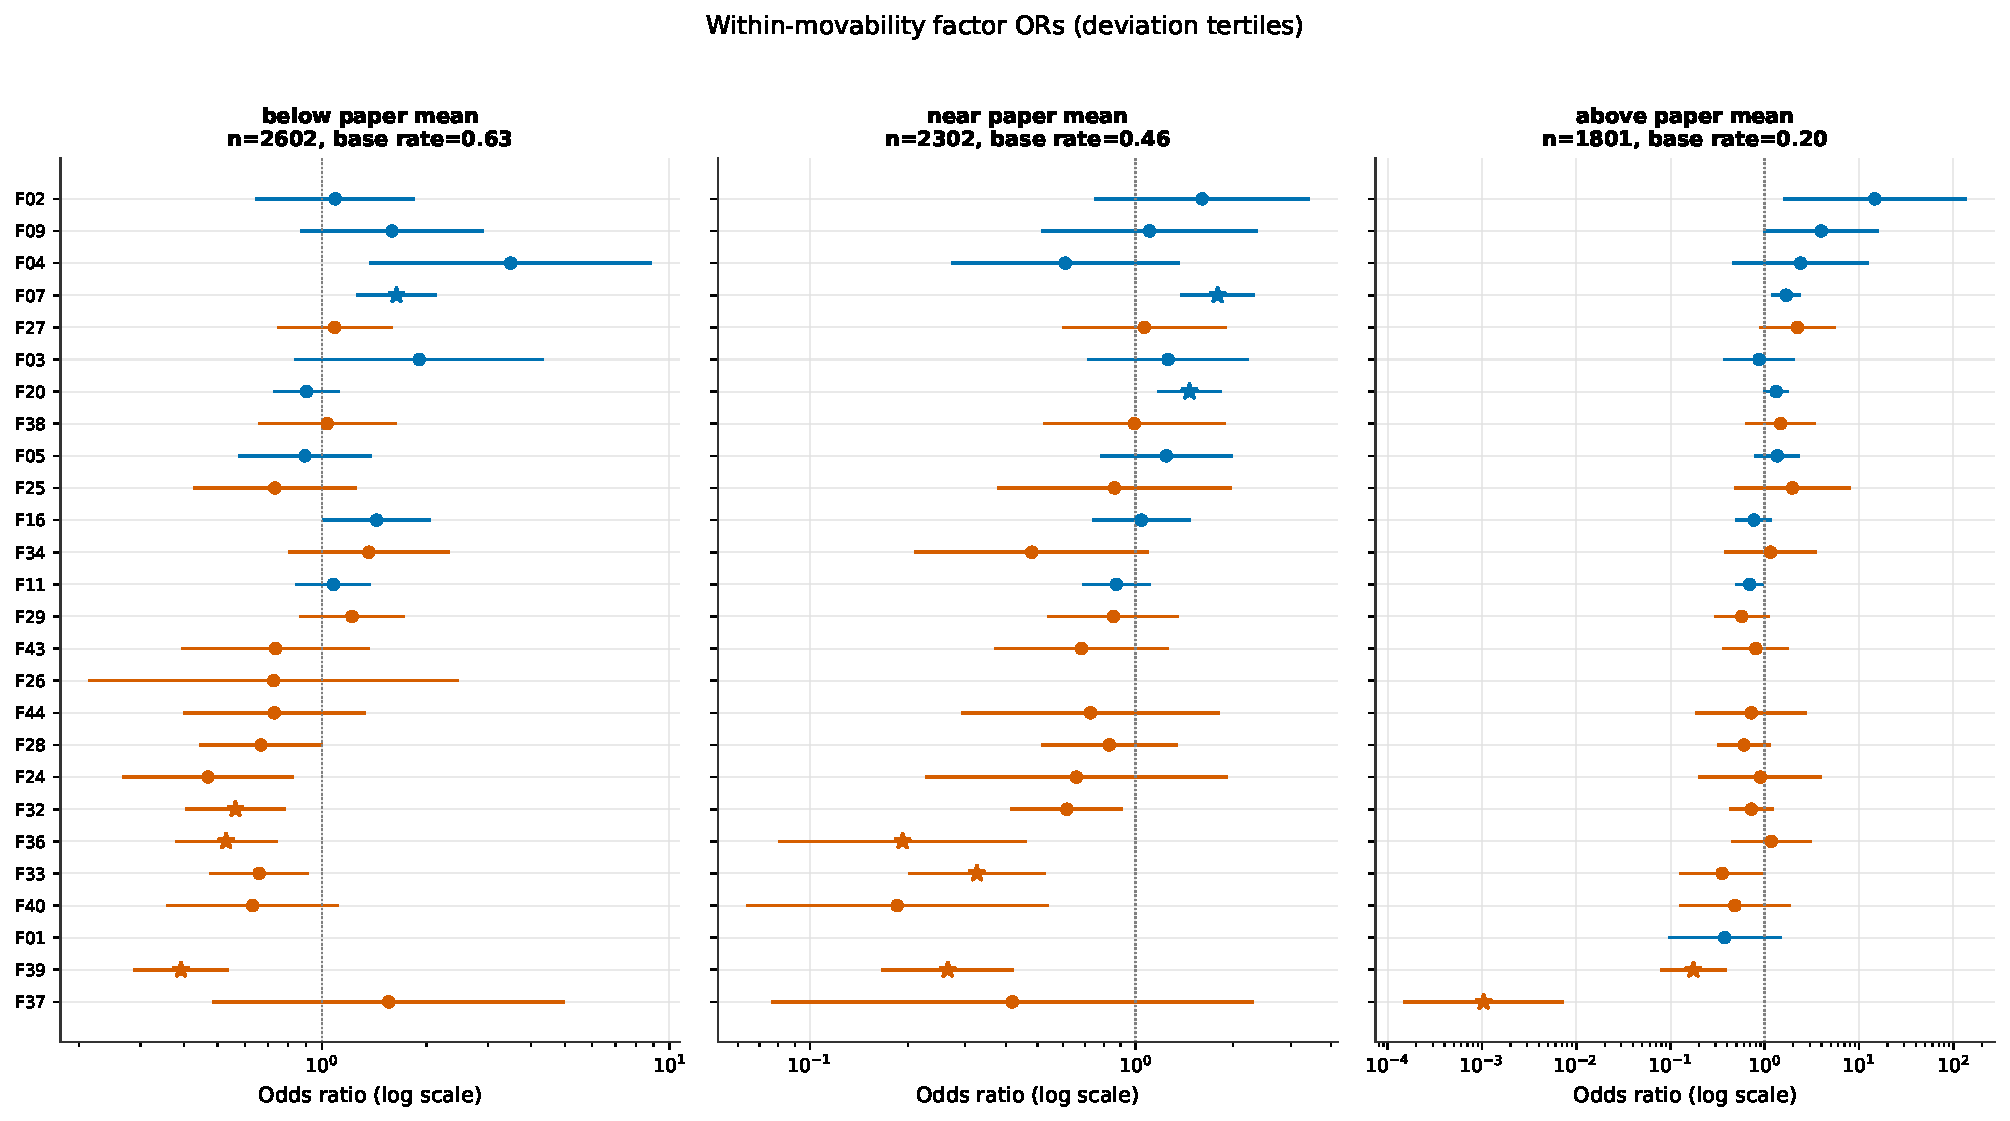
\includegraphics[width=0.85\linewidth]{../../data/results/horizon_inference/figures/forest_movability_strata.pdf}
  \caption{\textbf{Rebuttal-content factors within fixed movability strata.} Three panels show the same headline logistic refit on the cohort split by reviewer deviation from the paper-level initial mean: below paper mean ($\code{deviation} \le -0.5$, $n=2{,}602$, base rate $62.8\%$), near paper mean ($|\code{deviation}| < 0.5$, $n=2{,}302$, base rate $46.0\%$), and above paper mean ($\code{deviation} > 0.5$, $n=1{,}801$, base rate $20.2\%$). Markers: blue = positive polarity, orange = negative; $\star$ = crosses Bonferroni at $\alpha = 0.05/44 = 0.0011$ within the stratum, $\circ$ otherwise. Y-axis lists factors with $|\log \text{OR}| > 0.3$ in any stratum (sorted by mean log-OR across strata). $F_{07}$ baseline completion and $F_{39}$ defensive responses keep their direction in all three strata; the above-paper-mean stratum has wider CIs because few rebuttals there end in a score increase at all.}
  \label{fig:movability-strata-app}
\end{figure}

\paragraph{Calibration on out-of-time data.} The same rebuttal-content logistic, refit on the year-$2024$ cohort only ($n = 5{,}710$) and evaluated on the year-$2025$ stratified slice ($n = 995$), produces predicted probabilities whose decile-binned means agree with the observed score-increase rate to within $\sim 0.05$ at the extremes (top decile predicted $0.94$ / observed $0.92$; bottom decile predicted $0.05$ / observed $0.15$) but with up to $\sim 0.20$ over-prediction in two middle deciles (predicted $\sim 0.65$ / observed $0.45$ and predicted $\sim 0.85$ / observed $0.75$). The 2025 slice is the stratified \Cref{res:rebuttal-categories} (Test 1) sample, balanced across tier and verdict-group rather than naturally distributed. The bin-level observed rates are therefore noisy and cannot be reweighted to a population estimate without revisiting that stratification. Binned numbers: $\code{calibration\_temporal.csv}$.

\paragraph{Threshold metrics at $0.5$.} The headline cascade in \Cref{sec:rebuttal-impact} reports rank-based metrics ($\auc$, $\auprc$). For readers who want a directly interpretable success/no-success readout we additionally report accuracy, precision, recall, and $F_1$ at a fixed decision threshold of $p = 0.5$ for the rebuttal-content model (\Cref{tab:threshold-metrics}). On the temporal split (train year-$2024$, predict year-$2025$ stratified slice), the logistic reaches accuracy $72.6\%$ ($F_1 = 0.71$) against a $44.4\%$ base rate; under paper-clustered $\texttt{GroupKFold}(5)$ on the full $n = 6{,}705$ pool, accuracy reaches $77.1\%$ ($F_1 = 0.75$). The random forest underperforms the logistic on every threshold-based metric as well, consistent with the rank-based result. Threshold-$0.5$ numbers under-use the model's information: the calibration plot shows the rank ordering is reliable across all deciles while the absolute probability scale is reliable mainly at the extremes, so reporting at a single threshold is informative for context only. Source: $\code{threshold\_metrics\_draft.csv}$.

\begin{table}[h]
  \centering
  \caption{Threshold-$0.5$ classification metrics for the rebuttal-content logistic and random forest. Temporal split = train year-$2024$, predict year-$2025$ stratified slice; GroupKFold(5) = paper-clustered out-of-fold predictions on the combined $n = 6{,}705$ pool. Confusion-matrix cells: $tn$, $fp$, $fn$, $tp$.}
  \label{tab:threshold-metrics}
  \footnotesize
  \begin{tabular}{llrrrrrrrrrr}
    \toprule
    Split & Model & $n$ & base & acc. & prec. & recall & $F_1$ & $tn$ & $fp$ & $fn$ & $tp$ \\
    \midrule
    Temporal $2024 \to 2025$ & Logistic       & 995  & 0.444 & 0.726 & 0.666 & 0.767 & 0.713 & 383  & 170 & 103 & 339  \\
    Temporal $2024 \to 2025$ & Random forest  & 995  & 0.444 & 0.718 & 0.671 & 0.715 & 0.692 & 398  & 155 & 126 & 316  \\
    GroupKFold(5)            & Logistic       & 6705 & 0.456 & 0.771 & 0.739 & 0.770 & 0.754 & 2817 & 832 & 703 & 2353 \\
    GroupKFold(5)            & Random forest  & 6705 & 0.456 & 0.762 & 0.739 & 0.740 & 0.739 & 2849 & 800 & 795 & 2261 \\
    \bottomrule
  \end{tabular}
\end{table}

\paragraph{Scenario demonstrations.} For \Cref{tab:scenarios} we construct a "median-2024 author profile" by taking the median (continuous) or majority value (binary) for each feature on the year-2024 cohort, then read off the predicted probability under the listed factor-presence overrides. The scenario predictions are derived from the calibration-tested model (year-2024 fit), not the headline combined-data fit. Numbers: $\code{scenario\_predictions.csv}$.

\paragraph{Reproduction.}
\begin{itemize}[itemsep=0pt,topsep=2pt]
  \item Cascade-prediction (logistic + RF, three horizons, temporal + GroupKFold): $\code{src/analyze/rebuttal\_rf\_prediction.py}$.
  \item Inferential analysis (paper-clustered logistic, marginal fits, ablations, recommendation gate, calibration, scenarios): $\code{src/analyze/horizon\_inference.py}$.
  \item Row-level factor labels: $\code{data/results/32\_factor\_taxonomy/interaction\_factor\_labels\_\{2024,2025\}.csv}$.
  \item Cascade tables and figures: $\code{data/results/rebuttal\_rf\_prediction/}$.
  \item Inferential tables and figures: $\code{data/results/horizon\_inference/}$.
  \item Leakage tests: $\code{tests/test\_horizon\_leakage.py}$.
\end{itemize}

\subsection{Confidence-and-trigger analysis}\label{app:confidence-triggers}

To analyse what is associated with score revision, we focused on below-mean outlier reviewers (those who scored a paper lower than the co-reviewer average) and grouped them by confidence level and score-change outcome. We tested four families of potential triggers:
\begin{itemize}[itemsep=0pt,topsep=2pt]
  \item \textbf{Peer alignment.} Reviewer deviation from paper mean (z-score within the paper's review panel) and co-reviewer movement (share of co-reviewers who also increased their score after rebuttal).
  \item \textbf{Rebuttal effort.} Author reply length (in words and characters), number of author replies, and total thread message count.
  \item \textbf{Review characteristics.} Sub-scores (soundness, contribution, presentation), strength and weakness text lengths.
  \item \textbf{Engagement quality.} LLM-extracted engagement and actionability ratings from review text.
\end{itemize}

\paragraph{Operational definitions.}
\textit{Outlier} = z-score $\le -1.0$ within the paper's review panel (${\sim}15\%$ of reviews). \textit{Long rebuttal} = top quintile of reply length (more than \num{1574} words or \num{7870} characters). \textit{Peer-movement bucket} = share of co-reviewers who increased their score after rebuttal, binned into \{0, 1--25, 26--75, 76--100\}\%. \textit{Low confidence} = self-reported reviewer confidence $\le 3$ on the 5-point ICLR scale.

\paragraph{Statistical tests.}
Two-group comparisons used Mann-Whitney $U$ with rank-biserial correlation as effect size. Multi-group comparisons used Kruskal-Wallis with epsilon-squared, followed by pairwise Mann-Whitney with Bonferroni correction. Year-stratified replications (2024 vs.\ 2025) are reported alongside the combined estimates. Source figures: \code{data/results/confidence\_triggers/figures/}.

\subsection{Rebuttal content coding: 44-factor taxonomy with cross-model validation}\label{app:rebuttal-coding}

The factor taxonomy was induced and validated in three stages: induction with LLM-A (Claude), independent classification with LLM-B (Gemini Flash 3), and a held-out replication test on disjoint data. Two conditions were declared at the start of the analysis: (a) the factors reflect structure in the interaction text rather than patterns internal to LLM-A, and (b) the factor-outcome associations replicate beyond the induction sample.

\paragraph{Sample for taxonomy induction.}
From ICLR 2025 we drew \num{1000} reviewer-paper pairs stratified by reviewer initial rating (low 1--3, medium 5--6, high 8--10) crossed with rebuttal outcome (\code{increase} vs.\ \code{same\_decrease}), restricted to pairs with a non-empty author rebuttal thread. Each pair was serialised as a raw text thread containing the full original review (summary, strengths, weaknesses, questions), the full author rebuttal, and any reviewer follow-up comments, in chronological order. No structured Gemini-extracted fields (sentiment, tone, engagement-quality, score-change verdict outputs) were exposed to either LLM-A or LLM-B at any point in this analysis. The serialised threads are shipped at \code{data/results/factor\_validation/induction\_input\_1k\_threads\_iclr2025.json}. The high-increase cell is rare in ICLR 2025. We therefore used all 58 available pairs rather than subsample, which matches the strategy later applied to the ICLR 2024 hold-out. The remaining five cells were filled by random sampling.

\paragraph{Factor induction (LLM-A = Claude).}
In a single prompt we presented LLM-A with all six cells of the sample and instructed the model to perform the contrast within each tier (low-\code{increase} vs.\ low-\code{same\_decrease}, and analogously for medium and high). The within-tier framing preserves tier-specific patterns and prevents the model from collapsing the task into a single cross-tier contrast that could be dominated by score-level differences rather than rebuttal content. We repeated the procedure five times to attenuate run-to-run variability, then manually aggregated the extracted categories across runs and tiers, merging entries that were pure rephrasings or semantically close. The aggregation yielded 44 factors, each labelled with a declared polarity (positive or negative) from the pooled induction output.

\paragraph{Memory-control swaps.}
To rule out the hypothesis that LLM-A was retrieving canonical patterns from its prior rather than reading the interactions, we re-ran the induction under two manipulations. The first swapped the low-tier and high-tier interactions within the same prompt structure. The second silently swapped the \code{increase} and \code{same\_decrease} outcome labels on the same \num{1000} interactions, holding tier assignment fixed. In both cases the resulting factor content shifted with the presented inputs rather than tracking the labels, consistent with extraction from the interaction text. The outcome-label swap (the sharper of the two stress tests, since it operates on the axis the original induction used to discriminate) confirms that LLM-A continues to locate the same features on the same actual data even when the labels are flipped, and only the surface narrative re-frames around the new labels.

\paragraph{Classification protocol (LLM-B = Gemini Flash 3).}
A second, independent Gemini call classified each interaction against the fixed 44-factor list. The classifier saw the same raw thread text used at induction (no structured features), the 44-factor codebook with shuffled per-request factor identifiers, and the request to mark which factors were present. Classification was outcome-blinded: reviewer tier and rebuttal outcome were stripped from the prompt, factor identifiers were shuffled per request so that ordering could not cue the model, and the Gemini response schema constrained each returned \code{factor\_id} to the set F01--F44, blocking hallucinated categories. For every factor we computed an odds ratio comparing the \code{increase} and \code{same\_decrease} outcome groups, with a 95\% confidence interval, and a two-sided permutation test with 2000 permutations. Under each permutation the \code{increase} / \code{same\_decrease} labels are randomly reshuffled across interactions to simulate the null of no factor-outcome association, the odds ratio is recomputed, and the $p$-value is the fraction of shuffles whose $|\log \text{OR}|$ matches or exceeds the observed value (with add-one smoothing to keep $p > 0$). Significance is reported at the Bonferroni-corrected threshold $\alpha = 0.05 / 44 = 0.0011$. Choosing 2000 permutations gives a resolution floor of about $1/2001 \approx 0.0005$, just below the Bonferroni-corrected threshold.

\paragraph{Choice of multiple-testing correction.}
Bonferroni is the most stringent of the standard family-wise error-rate (FWER) controls and assumes nothing about test independence. We anchor on it because the held-out replication on a disjoint ICLR 2024 sample (Test 2) is itself a strong robustness check that partially substitutes for relaxing within-test correction, and because surviving the strictest correction leaves least room for over-claiming. Two alternative corrections are reasonable to consider, both more permissive (\Cref{tab:mtcorrection}). Holm-Bonferroni controls the same FWER as Bonferroni but is uniformly more powerful (it never rejects fewer hypotheses); it yields 18 doubly-significant factors instead of 16. Benjamini-Hochberg FDR controls the expected proportion of false positives \emph{among the rejected} hypotheses (a weaker but often more appropriate guarantee for discovery-style analyses) and at $q = 0.05$ yields 26 doubly-significant factors. Direction of effect agrees with the Bonferroni-anchored core in all three views; the more permissive corrections add factors to the core rather than displace any of its members.

\begin{table}[htbp]
    \centering
    \caption{Sensitivity of the doubly-significant factor count to the multiple-testing correction. Bonferroni is the headline reported in \Cref{res:rebuttal-categories}.}
    \label{tab:mtcorrection}
    \begin{tabular}{lccc}
    \toprule
    Correction & Test 1 & Test 2 & In both \\
    \midrule
    Uncorrected $p < 0.05$              & 32/44 & 43/44 & --- \\
    Bonferroni $\alpha = 0.05 / 44$    & 23/44 & 40/44 & \textbf{23/44} \\
    Holm-Bonferroni $\alpha = 0.05$    & 25/44 & 42/44 & 25/44 \\
    Benjamini-Hochberg $q = 0.05$      & 31/44 & 43/44 & 31/44 \\
    Benjamini-Hochberg $q = 0.10$      & 32/44 & 44/44 & 32/44 \\
    \bottomrule
    \end{tabular}
\end{table}

\paragraph{Tests.}
\textbf{Test 1 (operationalisability)} applies LLM-B to the same \num{1000} ICLR 2025 interactions used for induction, asking whether a second model can recover the induced factors from the same text. \textbf{Test 2 (discriminative validity)} applies the same protocol to the full classified ICLR 2024 cohort of \num{5730} interactions disjoint from the induction corpus, asking whether the factor-outcome associations replicate on fresh data. An earlier round of Test 2 was reported on a \num{952}-interaction stratified subsample of the same cohort (six-cell stratification by tier and verdict-group); the conclusions of that smaller test (43 of 44 codebook polarities preserved, 16 of 44 doubly-Bonferroni-significant) hold under the present full-cohort version, with strict strengthening on every count. Source: \code{src/factor\_validation/expand\_test2\_full2024.py}; comparison CSV: \code{test2\_full2024\_comparison.csv}.

\paragraph{Cohort thinness and clustering.}
The classified ICLR 2024 cohort contains \num{5730} rebuttals across \num{3460} unique papers, an average of $1.66$ rebuttals per paper. This is a thinned slice of ICLR 2024's natural ${\sim}4$-reviewer paper structure, because not every reviewer wrote a rebuttal and not every (paper, reviewer) pair survived Gemini classification. The headline Test 2 permutation test uses naive (row-level) shuffling, matching the protocol used for the original Test 1 / Test 2 pair. As a robustness check we re-ran the expanded Test 2 with a within-paper block permutation that swaps outcome blocks at the paper level. The doubly-Bonferroni-significant count is unchanged at $23$ and per-factor $p$-values agree to within $0.005$. We do not lean on the block-permutation result as a paper-clustered correction in the body text, because the cohort thinness limits how much within-paper correlation our block test can detect, and we cannot rule out residual within-paper correlation in unobserved rebuttals or selection bias in which (paper, reviewer) pairs produced a classified rebuttal.

\paragraph{Results.}
The taxonomy shows the declared directional structure in both tests. In Test 1, 43 of 44 factors are more prevalent on the side of the \code{increase} versus \code{same\_decrease} contrast declared at induction (22 of 23 positive, 21 of 21 negative), and 23 of 44 survive the Bonferroni threshold. In Test 2, all 44 of 44 factors match their declared direction (23 of 23 positive, 21 of 21 negative), and 40 of 44 individually survive Bonferroni at the full-cohort sample size. The single Test 1 disagreement is F12 (proactive limitation acknowledgement) inverting polarity with OR = 0.90 [0.68, 1.19]; under the original \num{952}-interaction Test 2 subsample, F40 (marginal quantitative improvements) was the corresponding inversion at OR = 1.52 [0.76, 3.05], but it lands at OR = 0.36 [0.26, 0.51] in the full cohort, matching its declared negative polarity. Of the 44 factors, 23 cross Bonferroni in both tests (9 positive, 14 negative) and form the conservative core of the taxonomy. No factor crosses only in Test 1, and a further 17 cross only in Test 2 (the larger sample resolves several borderline factors that the in-sample run lacks power to detect). These are retained but reported as weaker evidence.

\begin{table}[htbp]
  \centering
  \caption{The 23 doubly-significant factors that anchor the taxonomy. ``Polarity'' is the direction declared at induction (LLM-A) and confirmed by both LLM-B tests at the Bonferroni-corrected threshold $\alpha = 0.05 / 44$.}
  \label{tab:taxonomy-core}
  \small
  \begin{tabular}{p{0.8cm} p{1.5cm} p{11cm}}
    \toprule
    \textbf{ID} & \textbf{Polarity} & \textbf{Label} \\
    \midrule
    F02 & positive & Non-defensive, respectful, collaborative tone. \\
    F04 & positive & Sincere engagement: detailed responses, length, added appendix content. \\
    F05 & positive & Methodological detail and reproducibility clarification. \\
    F06 & positive & Concrete empirical evidence tied to reviewer concerns. \\
    F07 & positive & Baseline completion / comparator strengthening. \\
    F13 & positive & Explicit manuscript revision signaling. \\
    F14 & positive & Supplementary material and new visual evidence. \\
    F21 & positive & Active dialogue and continued engagement. \\
    F22 & positive & Concrete revision commitments. \\
    \midrule
    F24 & negative & Defensive or dismissive tone. \\
    F25 & negative & Superficial or partial addressal of reviewer concerns. \\
    F27 & negative & Missing or insufficient baseline comparisons. \\
    F28 & negative & Lack of quantitative / empirical evidence in rebuttal. \\
    F29 & negative & No new requested experiments / analyses / ablations. \\
    F30 & negative & Vague future-oriented promises instead of concrete commitments. \\
    F31 & negative & Narrow or insufficient evaluation scope. \\
    F32 & negative & Incomplete empirical coverage even after rebuttal additions. \\
    F33 & negative & Unresolved quality-of-execution concerns that further experiments do not fix. \\
    F36 & negative & Weak novelty justification. \\
    F38 & negative & Section-referencing or paper-rephrasing instead of real clarification. \\
    F39 & negative & Inadequate explanation or persistent clarity issues. \\
    F42 & negative & Vague or insufficient technical explanation. \\
    F43 & negative & No explicit commitment to revise or improve the paper. \\
    \bottomrule
  \end{tabular}
\end{table}

Source: \code{data/results/factor\_validation/}. Induction prompt and classification prompt are reproduced verbatim in \Cref{app:prompts}.

\subsection{Statistical framework}\label{app:stats}

We use non-parametric tests throughout, given the discrete and ordinal nature of reviewer ratings (six-point scale with uneven spacing \{1, 3, 5, 6, 8, 10\} for 2023 to 2025; see \Cref{app:dataset}). For two-group comparisons we use Mann-Whitney $U$ with rank-biserial correlation as effect size. For multi-group comparisons, Kruskal-Wallis with epsilon-squared. For correlations involving the score or confidence scales we report Spearman $\rho$ rather than Pearson $r$. Pearson's magnitude depends on the (arbitrary) numeric spacing of the scale, while Spearman, being rank-based, is invariant to it. For binary outcomes we use chi-squared or Fisher's exact tests with Cramer's V as effect size, and logistic regression with cluster-robust standard errors (statsmodels \code{cov\_type='cluster'}, \code{cov\_kwds=\{'groups': paper\_key\}}). For count data we use Mann-Whitney $U$ or Poisson / negative binomial regression.

We adopt a significance threshold of $p < 0.001$ throughout and prioritise effect sizes over $p$-values, since with $n > \num{70000}$ even trivial differences reach statistical significance. Bonferroni correction is applied to families of related tests (e.g., $8 \times 3 = 24$ tests for content-coding category by tier in \Cref{app:rebuttal-coding}). All claims use predictive language (``associated with'', ``predicts'', ``co-occurs with''). We do not claim causation. Reviews within a paper are not independent (reviewers read the same manuscript and observe each other's scores during discussion), so all prediction models use \texttt{GroupKFold} by \code{paper\_key} and all regression coefficients use cluster-robust standard errors clustered on \code{paper\_key}.

An inclusion funnel (\Cref{app:dataset}) documents the sample attrition at each analysis stage. Balance checks confirm that retained and excluded subsets do not differ systematically on initial score, confidence, or acceptance rate.

\subsection{Prompts}\label{app:prompts}
% Verbatim text:
%   - src/prompts/classification_instruction.py (Gemini score-prediction prompt)
%   - src/prompts/categorization_prompt.py     (rebuttal content coding)
%   - any factor_validation prompt(s)
% Include input schema and JSON output schema for each.

\subsection{Reproducibility}\label{app:repro}

Pipeline commands are wrapped in a Makefile in the project root: \code{make all-local} runs the full pipeline assuming raw data and batch outputs are present, \code{make analyze} runs the analysis scripts only, and \code{make figures} regenerates publication figures. The Python environment is captured in \code{requirements.txt}.

\paragraph{Random seeds.}
All sampling uses \code{random.seed(50)} (\code{src/core/sampling.py}: \code{get\_sampled\_indices(population, k, seed=50)}). The 1K validation sample described in \Cref{app:score-change} uses this seed.

\paragraph{Batch outputs and a data-integrity note.}
The full ICLR 2024 Gemini prediction file (\code{gemini\_3flash\_iclr2024\_full.json}) was originally produced by 25 chunked batch jobs. An early invocation of the \code{download-all} command before all chunks had completed left the assembled file with only 962 papers, corresponding to a 13.2\% review coverage. The file was subsequently rebuilt from all 25 chunks, yielding the correct 7,262 papers and 99.7\% review coverage. All numbers reported in the present paper use the rebuilt file.

\paragraph{Pipeline phases.}
Six numbered phases under \code{pipeline/} encode the dependency graph: collect ($\to$ raw JSON), normalise ($\to$ \code{data/processed/normalized/}), predict (Gemini batch submission and download), detect score changes (regex + Gemini verdict), analyse (the scripts under \code{src/analyze/}), and figures (the notebooks that produce the publication-ready PNG/PDF pairs in \code{data/results/figures/}). The \code{Makefile} encodes the dependencies between phases.

\end{document}
